% !TEX TS-program = pdflatex
% !TEX encoding = UTF-8 Unicode

%tells you if you use obsolete packages
%\RequirePackage[l2tabu,orthodox]{nag}

\documentclass[]{article}

\usepackage[utf8]{inputenc} % set input encoding (not needed with XeLaTeX)
\usepackage[T1]{fontenc}

\DeclareUnicodeCharacter{00A0}{ }

%%% PAGE DIMENSIONS
\usepackage{geometry} % to change the page dimensions
\geometry{a4paper} % or letterpaper (US) or a5paper or....
\geometry{margin=1in} % for example, change the margins to 2 inches all round
% \geometry{landscape} % set up the page for landscape
%   read geometry.pdf for detailed page layout information

\usepackage{graphicx} % support the \includegraphics command and options

% \usepackage[parfill]{parskip} % Activate to begin paragraphs with an empty line rather than an indent

%%% PACKAGES
\usepackage{booktabs} % for much better looking tables
\usepackage{array} % for better arrays (eg matrices) in maths
\usepackage{paralist} % very flexible & customisable lists (eg. enumerate/itemize, etc.)
\usepackage{verbatim} % adds environment for commenting out blocks of text & for better verbatim
\usepackage{subfig} % make it possible to include more than one captioned figure/table in a single float
%auto expansion is only possible with scalable fonts\usepackage{microtype} %makes awesome kerning and punctuation come half way out the edge of the text
\usepackage{listings} %for code listings
\usepackage{color} %for colored syntax highligting
\usepackage{rotating}
\usepackage{pdflscape}
\usepackage[]{algorithm2e}
\usepackage{multirow}
\usepackage{float}
\usepackage{mathtools}
\usepackage{amssymb}



\usepackage{caption}
% \captionsetup[subfigure]{format=subfig,labelsep=colon,labelformat=simple}
% \usepackage{subcaption}

\usepackage[backend=bibtex, bibencoding=utf8]{biblatex}
\bibliography{biblib} 
%%% Code listing
\definecolor{mygreen}{rgb}{0,0.6,0}
\definecolor{mygray}{rgb}{0.5,0.5,0.5}
\definecolor{mymauve}{rgb}{0.58,0,0.82}
\lstset{
basicstyle=\footnotesize\ttfamily,
commentstyle=\color{mygreen},
keywordstyle=\color{blue},
numberstyle=\tiny\color{mygray},
numbers=left,
tabsize=2,
frame=tb,
aboveskip=3mm,
belowskip=3mm,
breaklines=true,
breakatwhitespace=true,
showstringspaces=false,
columns=flexible
}

% to include a file as a listing: \lstinputlisting{intio.c}
% inline listing: \begin{lstlisting}[frame=single]

%%% HEADERS & FOOTERS
\usepackage{fancyhdr} % This should be set AFTER setting up the page geometry
\pagestyle{fancy} % options: empty , plain , fancy
\renewcommand{\headrulewidth}{0pt} % customise the layout...
\lhead{}\chead{}\rhead{}
\lfoot{}\cfoot{\thepage}\rfoot{}

%%% ToC (table of contents) APPEARANCE
\usepackage[nottoc,notlof,notlot]{tocbibind} % Put the bibliography in the ToC
% \usepackage[titles,subfigure]{tocloft} % Alter the style of the Table of Contents
%\renewcommand{\cftsecfont}{\rmfamily\mdseries\upshape}
%\renewcommand{\cftsecpagefont}{\rmfamily\mdseries\upshape} % No bold!
\usepackage{hyperref} % use hyperlinked ToC
\hypersetup{colorlinks=true, linkcolor=black, citecolor=black, filecolor=black, urlcolor=black}
\graphicspath{ {ImageLib/}{other_folder/}{third_folder/} }

\usepackage[printonlyused]{acronym}

%%%-------------------------------------------------------------------


\title{Third Year Group Project \\ State Estimation for Indoor Environments}
\author{Oskar Weigl, Ryan Savitski, Thomas Morrison, Chinemelu Ezeh, Joshua Elsdon}
\begin{document}
\maketitle
\center{\textbf{\large{\emph{"...a profound trust in the advances of science."}	}}}

\abstract{
A Lovely Abstract full of insight and long words that makes it apparent we did lots of stuff 
\tableofcontents
\clearpage

\section{Acronyms} % (fold)
\label{sec:acronyms}
\begin{acronym}[DBScan]
	\acro{UAV}{Unmanned Aerial Vehicle}
	\acro{MAV}{Micro Aerial Vehicle}
	\acro{EKF}{Extended Kalman Filter}
	\acro{DoF}{Degrees of Freedom}
	\acro{MMSE}{minimum mean square error}
	\acro{PCL}{point cloud library}
	\acro{DBScan}{density based scan}
	\acro{PCA}{principle component axis}
	\acro{GPS}{Global Positioning System}
	\acro{RGB}{Red Green Blue}
	\acro{RGB-D}{Red Green Blue - Depth}
\end{acronym}
\clearpage
% section acronyms (end)

\section{Executive Summary} % (fold)
\label{sec:executive_summary}
\subsection{Introduction}
In the present world of increasing machine usage and autonomy, it is important for robots to be able to correctly estimate their position, velocity and in general their current state at any given time in order to perform tasks with much better accuracy. For our project we focused on determining the indoor state also known as the indoor localisation problem of quadcopters. Quadcopters have become a famous hobbyist platform but more importantly, they can be used in autonomous rescue operations and aerial photography. Our project is in essence a first step towards implementing indoor simultaneous localisation and mapping (SLAM). With this in mind, we served as consultants to a start up company called MAVRX who specialises in developing unmanned aerial vehicles(UAVs), supporting electronics and software. Our mission is to enhance MAVRX's interest and research by developing an indoor state estimator that can be used for autonomous quadcopters. They in turn provide us with necessary tools including an R10 quadcopter, a wireless remote controller, and basic code for stabilising and controlling the UAV.
\subsection{Our Solution}
While there has been lots of work done in the area of localisation, we propose a unique solution targeting indoor environments which consists using on-board processing and RGB-D cameras as our primary sensor combined with accelerometer and gyroscope sensors capable of working in GPS deficient areas. Our approach leverages the powerful yet cheap capabilities of the Xtion Pro camera. A typical solution to localisation involves modelling the motion of the agent as it moves in the environment, extracting features from the environment using sensors and using this information to approximate its location within the environment. We decided to track wall planes as our feature extracting plane equations from the Xtion Pro using DBSCAN algorithm because of the algorithm's resistance to noise and bounded-time operation. Moreover, Using an RGB-D camera provides lots of information and is resistant to interference compared to sonar sensors. For the actual state estimation, we employ the kalman filter algorithm as it produces optimal solutions in the presence of noise.  
\subsection{Results}
Using DBSCAN algorithm, we were able to extract planes as features. Observing three orthogonal planes provide full observability in the x, y and z axis. Using the extended kalman filter, we were able to show that our system can estimate its position, velocity and attitude in an indoor environment. We had to tune the filter providing empirical values for uncertainties in the Xtion's observation obtained through numerous testing. We confirmed the consistency of our filter by checking for bias in its measurement error and ensuring its boundedness is described by its covariance. Our system gave us accurate positioning(with 10mm precision) verified using a measuring tape. 

\subsection{Conclusion}
Localisation and state estimation is a first step towards full autonomous simultaneous localisation and mapping which combined with the high maneuverability of the quadcopter opens up new areas in robotics. We have thus pushed forward a bit the goal of our client company, Mavrx in developing unmanned aerial vehicles. Our project has shown and demonstrated the possibilities of indoor state estimation without GPS data which has commercial benefits in the aerial photography market as well as applications in search and rescue operations. Our system can be applied in the industry where aerial monitoring is essential such as pipeline inspection and area mapping.  

\clearpage

\section{Problem Specification}
\label{sec:problem_specification}

\subsection{Project Aim}
\label{sub:what_are_we_trying_to_achieve}
\cite{OpenPilotinsgps}
This project aims to provide our client with a functional prototype of an autonomous flying platform, much like a traditional \ac{UAV}. The novel aspect of this prototype will be the fact that it can operate in \ac{GPS} denied environments, such as indoors and in urban canyons. The aim of the prototype is to be a proof of concept, showing that with current technology, a flying robot can be autonomous in \ac{GPS} denied environments using only on-board sensors and computing. 

There are often situations where unmanned aerial vehicles could be useful, such as: search and rescue; infrastructure inspection (power lines, sewers); photography and videography. These tasks are already performed routinely by \ac{UAV}s, though usually controlled remotely by a human operator. In some cases the human operator is removed, and \ac{GPS} is used to close the loop on absolute positioning. This is a great solution for many problems, as it is quite cheap and can work nearly anywhere in the world. There are some places though where \ac{GPS} will not work reliably, such as inside a building or between many tall buildings (often called an urban canyon). These environments also would put pressure on the skill of a human operator due to the abundance of obstacles. Therefore providing a system that can reliably navigate indoors without a human operator is a very good idea. 

\subsection{Who are MavRX and Why are They Interested?} % (fold)
\label{sub:why_are_mavrx_interested_in_this_work_}

MavRX are a small start-up firm that are trying to push the frontiers of affordable \ac{UAV}s for the masses. Having achieved massive success in crowd-funding a cheap quadcopter platform, they are looking at pushing into more novel areas of \ac{UAV} production. They have asked us to help pave the road to a fully autonomous flying platform that will be priced in the consumer range rather than military/defence category like similar autonomous platforms. The main thing they are interested is a proof of concept model that they can use to attract support and funding with, as well as using it as a base for future experimentation. We must also give some thought to the pricing of the hardware to ensure we are not developing an infeasible product, though MavRX do not want us to spend much time on pricing and comparison of components, nor to develop a financial plan for this project as they already have a team of people working on the business aspect of this project.  

\subsection{Other Work in This Field} % (fold)
\label{sub:other_work_in_this_field}

This section will explore solutions to this and similar problems generated by other academics. The approaches to localisation for \ac{UAV}s and \ac{MAV}s (Micro Aerial Vehicles) fall into 3 main categories: Optical flow tracking \cite{DBLP:conf/icra/GrabeBG12}; time of flight laser scanners \cite{Bry2012} and rgb-d cameras \cite{Shen2012}.

Grabe et al\cite{DBLP:conf/icra/GrabeBG12} produced an interesting \ac{UAV} that uses a downward facing \ac{RGB} camera on a quadcopter to correct for sensor drift. This approach has a number of advantages firstly is the low cost of the hardware, \ac{RGB} cameras are now so common place that their price can be very low. In combination with other cheap sensors such as gyros, accelerometers, magnetometers and barometers a complete navigation solution becomes quite affordable. Though there are some significant downsides to this approach. Firstly there is no easy way to extract absolute data from the system, the concept of an absolute distance must be derived from the inertial sensors at some point, hence the whole system could be susceptible to drift over time. The conclusion of this paper suggests that this system would be well applied as a backup for a more robust tracking system. Therefore for now we can dismiss the use of optical flow tracking as a primary localisation technique. 

Bry et al. \cite{Bry2012} took a different approach. They used A fixed wing model aircraft and a planar time of flight (ToF) range finder for their localisation scheme. The use of a fixed wing aircraft offers one main advantage; high efficiency, therefore long flight times compared to a rotary aircraft such as a helicopter or quadcopter design. The draw back is that a fixed wing aircraft must be continually moving in order to stay airborne, and hence is more restrictive in environments that are confined. The ToF range finder is a very promising technology for localisation, it provides accurate data at high update rates. There are, as always, a number of issues; These range finders are very expensive, the one used here is \$5590 (Via Acroname Robotics)%http://www.acroname.com/robotics/parts/R314-HOKUYO-LASER4.html)
This is likely to put it out of contention for our project. Furthermore, these range finders only scan in one plane, hence only return quite sparse data. In order to identify features one must accumulate data along many planes, which depending on feature type, may make detection time prohibitively long. 

Shen et al. \cite{Shen2012} used a quadcoptor airframe and a \ac{RGB-D} camera from Microsoft combined with a laser range finder for localisation. Using the Depth channel of the camera they extract point cloud data to form an occupancy map and localise using the laser scanner. The benefit of the \ac{RGB-D} camera is that due to Microsoft pushing this technology to consumers, the sensors are considerably cheaper than the competition (\pounds 129.99). The laser range finder is used in a similar way to the above methods. Our implementation would not need the high density occupancy data that a full point cloud gives, a better use of this sensor may be to use it as the primary localisation sensor.

\subsection{Our Solution to the Problem} % (fold)
\label{sub:our_solution_to_the_problem}

Our solution is to use an \ac{RGB-D} camera as our primary sensor, supplemented with accelerometers and gyros and a downward facing sonar sensor. In order to generate the estimate of our state we will use an \ac{EKF} to fuse all the data. In order to simplify our feature extraction we will only extract planes from the environment, this is because planes are easy to characterise from all directions as well as being a consistently available feature in man made environments. We will be using the Asus Xtion Pro depth camera as our sensor as it is considerably lighter than the Microsoft Kinect, while maintaining a similar price point. Due to the somewhat narrow field of view we expect that the floor and the ceiling will often be out of view, hence reduced observability in the elevation direction. We will compliment the Xtion sensor with a downward facing sonar sensor, to address this issue.

With the above we can create a system that can accurately locate itself in a \ac{GPS} denied environment, and this will be satisfactory for MavRX to see the viability of the system. Though in order to get qualitative and quantitative data we wish to implement this system on an embedded platform on a \ac{MAV}. This will allow us to demonstrate the outcome of the project in a closed loop system and give MavRX valuable information about the utility of such a localisation system. 

For the embedded platform we have chosen to use a board called the 'arndale' board from INSIGNAL. This is due to its large amount of processing power and reasonably light weight design. It offers a dual core ARM A15 processor which will allow us to separate the two major tasks onto the different cores; feature extraction and Kalman filtering. 

We have decided to go with a quadcopter airframe for closed loop experimentation. This is because quadcopters have the ability to move around their environment slowly by hovering, this is especially useful when there is limited space for manoeuvre. Quadcopters also will have good stability, and therefore limit the amount of motion blur on the depth camera. Finally quadcopters are MavRX's speciality, so we will be able to make use of their expertise as well as helping them gather experience with this kind of air frame. 


% \subsubsection{Why did we Choose to Track Planes} % (fold)
% \label{ssub:why_did_we_choose_to_track_planes}

% \subsubsection{Why did we Choose the Xtion Sensor} % (fold)
% \label{ssub:why_did_we_choose_the_xtion_sensor}


% \subsubsection{Why did we Choose the Arndale Board} % (fold)
% \label{ssub:why_did_we_choose_the_arndale_board}

% \subsubsection{Why did we Choose a Quadcopter Platform} % (fold)
% \label{ssub:why_did_we_choose_a_quadcopter_platform}


% \begin{itemize}
% 	\item What are we trying to achieve
% 	\item Why is this a good idea to achieve
% 	\begin{itemize}
% 		\item why indoor navigation
% 		\item why are mavrx interested in this
% 		\item financial rundown (note that mavrx are intersted in a prototype consulting job, not a financial feasability report)
% 		\item discuss some of mavrx's buisiness model (if we are allowed)
% 	\end{itemize}
% 	\item What have other people done in this field
% 	\begin{itemize}
% 		\item insert papers here
% 	\end{itemize}
% 	\item how are we going to achieve it
% 	\item Why did we chose to do it that way
% 	\begin{itemize}
% 		\item why planes
% 		\item why xtion
% 		\item why arndale
% 		\item why quadcopter
% 	\end{itemize}
% \end{itemize}

% % section problem_specification (end)
\section{Implementation Overview}
\label{sub:implementation_overview}
Our state estimator involves a moving agent such as a quadcopter which deploys one sensor to gather information about its surroundings. This is called an exteroceptive sensor and in our case, we use a depth camera. We also incorporate extra sensors to measure the agent's own movement. These are called preprioceptive sensors and we used an accelerometer and a gyroscope. The state evaluation process involves the following steps:

\textbf{The agent moves, reaching a new point of view in the room} As a result of unavoidable noise
and errors, this movement increases the uncertainty on the robot's localization.
There is a need to model this motion to in implementing our state evaluation. This, we will call the motion model.

\textbf{The robot observes features in the room which need to be added to its interior map.} These features we call called landmarks. However, dues to errors in the depth camera, the location of the landmark will be uncertain. Moreover the robot's already uncertain position means that these two uncertainties have to be properly combined. We thus require a mathematical model to determine the position of the landmark from data obtained by the exteroceptive sensor. This we will call the inverse observation model.

\textbf{The robot re-observes landmarks and it uses them to  make corrections to its self-localisation and landmark position.} Thus reducing uncertainties on both. We also need a mathematical model to predict the values of the measurement from the predicted landmark location and the robot localisation. This will be the direct observation model.

The tasks can be group into two main categories feature extraction and extended kalman filter implementation.

\subsection{Feature Extraction}
The agent needs to properly observe its environment in order to be able to have some information of its relationship within the environment. First, we must chose a suitable sensor for our implementation taking into account the type of feature we want to extract. We chose to use a visual sensor/camera with depth information called the Xtion Pro as it is more more accurate and less prone to interference than using sound to observe the agent's environment. The camera essentially collects raw depth map data of 640 by 480 pixels at 30 frames per second. This is a huge amount of data to process especially in an embedded environment with limited resources. Moreover, the data in its raw form doesn't give much information in and off itself as it is only pixels with their depth information.

We use the Point Cloud Library (PCL) which is open source and is dedicated to processing such information from our xtion pro depth camera in order to perform a robust feature extraction process. With the PCL, we can extract feature of the indoor environment from the raw data of our camera. In selecting suitable features, we need them to be easily re-observable. With the assumption that our indoor environment is mostly cubic in nature, we decided to track walls, floors and ceilings as these are easily re-observable. Also, we can essentially represent a large wall as a plane and this requires minimal storage space as opposed to the millions of pixel data. This abstraction reduces considerably both computation and space complexity needed. The trade-off is .....
To extract planes, we employed the popular and much referenced density-based scan (DBScan) to cluster points in 3D in order to obtain the regression plane normal and distance information of the points. An alternative is to use the random sample consensus algorithm (RANSAC). There isn't however an upper bound time limit on the RANSAC algorithm while DBScan completes in $O(n^{2})$ time. In an embedded real-time environment with time constraints, an unbounded-time operation is not optimal. The planes produced are then sent to the extended kalman filter for state evaluation.

\subsection{Extended Kalman Filter}
The job of the extended kalman filter(EKF) is to perform an optimal evaluation of the robot's state given the presence of uncertainties in measurements. The EKF is a non-linear extension of the kalman filter which is itself a linear quadratic estimator capable of giving optimal values of a measurement in the presence of noise. Its results are more accurate than those obtained from single measurements. The EKF operates iteratively producing optimal values around the current mean and covariance. The other alternative to the EKF is the particle filter. The main difference is that the EKF produces optimal results using an approximate mathematical model while the particle filter produces optimal results based on physical models.
\cite{CompareFilters}Based on a comparative study on the difference between the two approached, for guassian noise model the kalman filter will always produce a better result in less computation time.

The state of the robot consists of its position, velocity, attitude, accelerometer bias, gyroscope biases  and landmark positions.The non-trivial state components, the biases due to heat variation and manufacture process errors are stored because they exhibit a random walk and thus depend on their previous values. \textbf{Insert reference for bias behaviour here}. The kalman filter iteratively update the robot's state along with its uncertainties called its covariance matrix.

The below image shows the basic concept of the EKF:
\begin{figure}[H]
\centering     %%% not \center
\subfloat[MATLAB]{\label{fig:kalman_pic}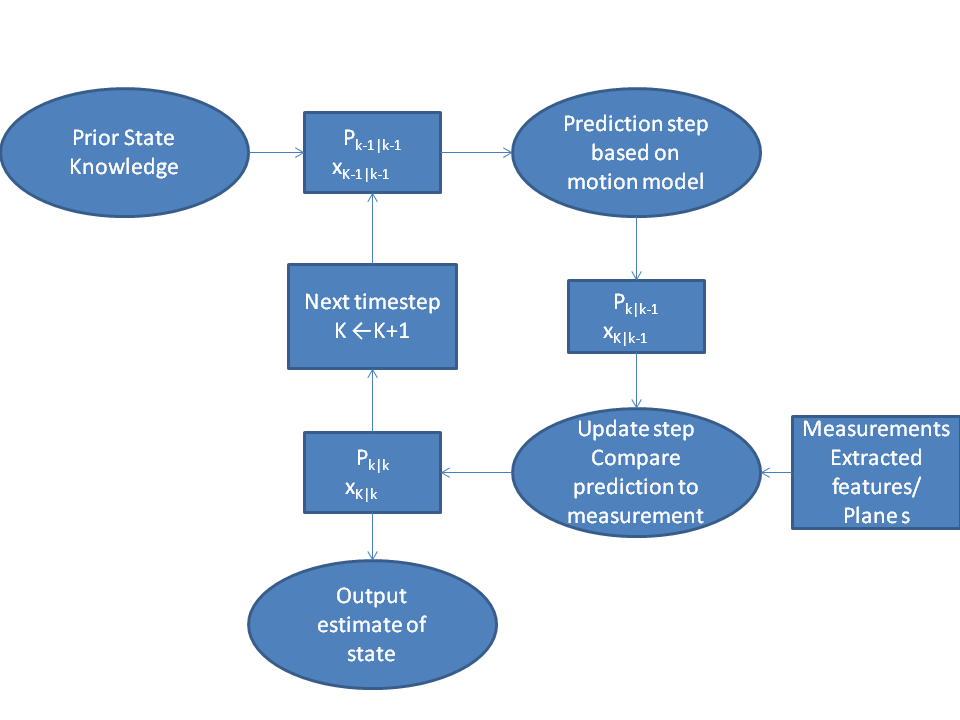
\includegraphics[width=60mm]{kalman_pic.PNG}} \;
\caption{Kalman algorithm Diagram}
\end{figure}

If more than one plane is observed, the update step is run for each plane re-observed. If a new plane is observed, it is added as a new landmark into the kalman filter and its covariance is added onto the covariance matrix.

\section{Preliminaries}
In this section, we discuss important procedures outside the main project implementation that has to be setup for the project implementation to work. This includes board selection, board configuration and Xtion sensor calibration. 
\subsection{System platform} % (fold)
\label{sub:system_platform}

((The project aims to implement the estimation algorithm on on-board processing.))

<<In choosing a platform to implement the algorithm, consideration needs to be given to the target processor's ISA and the operating system [[(or lack of thereof)]].>>

In conventional processor applications, <main consideration> is given to optimising the computational performance against cost and power usage. For an embedded system that is mounted on a quadcopter however, power usage of the chip is not a concern as it is not significant compared to the usage of the MAV itself. Therefore, for implementing this project we desire the best processing power per pound for the target workload. In this metric, no distinct advantage can be given to either of the two main standard processor architectures (x86 and ARM, including their derivatives) and the evaluation needs to be done on a chip-by-chip basis. 

In addition to the above, the choise of ISA is influenced by the support of the architecture by operating system support and the ability to interface with other system components that could be incorporated into the system (e.g. coprocessors). The target operating system for this project is a any lightweight distribution based on the linux kernel. This is due to the linux kernel being free, open source and being easily configurable, with the ability to compile in only the needed functionality and the ability to put options in loadable kernel modules. This results in an embedded operating system with minimal memory and processing footprint, as well as small disk usage which can be limited in embedded systems. For the specific libraries and frameworks used in implementing the estimation software (PCL and OpenNI), x86-Linux variants were found to have more mature support than ARM-Linux at the time of writing.

For low volume production, it is not always worth investing the engineering time in designing a custom system, sourcing the components and manufacturing. Instead, small form factor boards can be readily purchased at acceptable prices. [[include odroid u2 vs the atom board here as examples? Saying that both can handle the algorithm with less than N planes at sufficient frame rates to remain convergent and stable?]]

Additionally, we evaluated the possibility of using consumer smartphones as the embedded processing platform for the estimation algorithm. Android mobile operating system is built on top of the linux kernel and is also open source, making it the OS of choice for this comparison. The reasons for considering consumer smartphones are as follows:

- the smartphone market is extremely competitive, driving the prices down while improving the processing power to levels compatible with embedded systems usually seen in robotics applications.
- small form factor, including not needing big heatsinks.
- smartphones of all price ranges come with additional hardware and sensors that can be useful for the quadcopter platform. There are 9 DoF sensors in any device and USB functionality for interfacing to the RGB-D camera. Additionally, the estimation can be improved by using the phone's camera in a downwards looking configuration as an optical flow sensor. GPS can be used in semi-indoor environments and urban canyon situations. WiFi can be used to augment the system with wifi-slam [[http://www.tuaw.com/2013/03/23/wsj-apple-acquires-wifislam-indoor-location-tech-company/]] which gives additional localisation information for the system in indoor environments. Bluetooth can be used for [[???, short range wireless communication?]]. Furthermore, GPUs found in smartphones are starting to be OpenCL compatible (both Imagination Technologies' powerVR series and newer ARM Mali cores), which can provide easily accessible acceleration for certain parts of the algorithm.

However, in practice it was found that porting third party libraries used in the project and drivers for the RGB-D camera sensor, while possible, often needs significant engineering time spent. Additionally, the android platform enforces restricted APIs to underlying hardware resources, so it is not always possible to get the direct hardware control (e.g. for IMU) usually found in embedded linux systems.

[[price comparison of android phones with decent cpu vs embedded?]]

[[throw in fpga as additional possibilities, zynq7? :P, fixed point scaling blablabla]]

\subsection{Sensor Calibration} % (fold)
Apon inspecting the output of the Xtion Pro from Asus it became apparent that the accuracy of the data was poor as the sensor uses a logarithmic scale and not a linear one. At short ranges things appeared normal, and planes were indeed flat. At distance more than 2m planes quickly became warped (see Figure~\ref{fig:uncal5m}). This issue will corrupt the accuracy of planes that we extract from the cloud data, rendering the extra sensor of little use. 

\begin{figure}[H]
\centering     %%% not \center
\subfloat[MATLAB]{\label{fig:matlabuncal5m}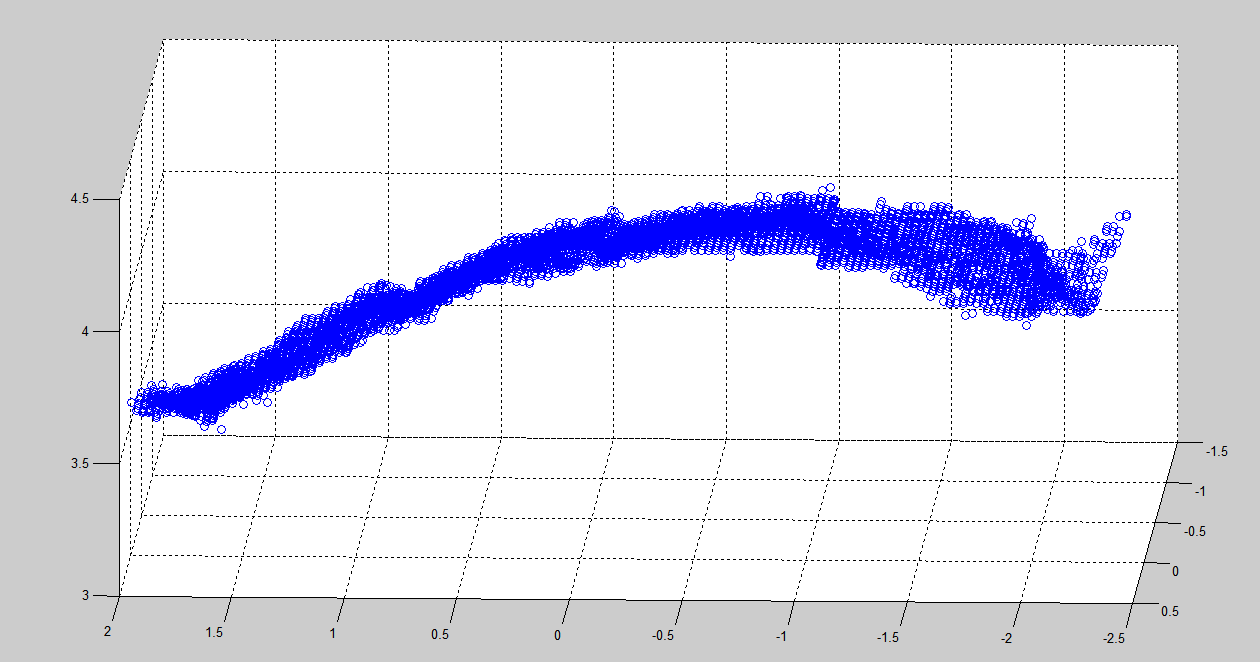
\includegraphics[width=60mm]{uncal5m.PNG}} \;
\subfloat[Colour Point Cloud]{\label{fig:clouduncal5m}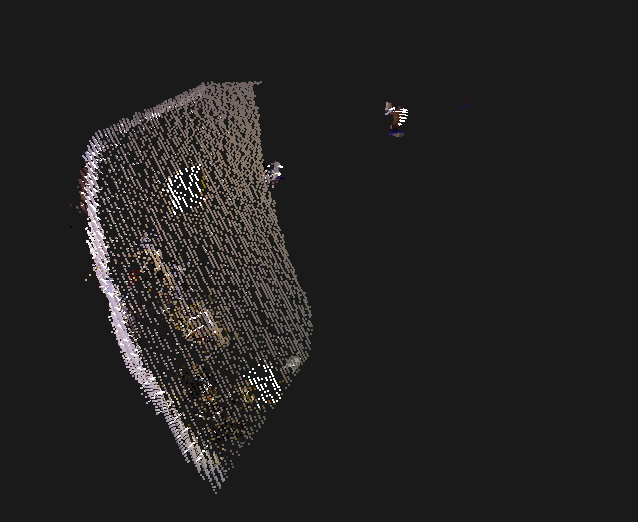
\includegraphics[width=60mm]{wallat6m}}
\caption{Example of the poor calibration of the Xtion sensor}
\label{fig:uncal5m}
\end{figure}


To attempt to counteract this issue we collected cloud data from when the sensor is facing a large plane, in this case a wall, at a number of distances (from 0.8m to 4m). This cloud data included lots of objects that are of no use to the calibration\textbf{(What do you mean by object and of no use?)}, so these data points were written to \verb"NaN" in the analysis to avoid corruption of our results. This was achieved by using the data written to an image file, with the z distance (down range from the camera) encoding the grey-scale. Then, by hand, we masked with black all the unwanted areas. This is then easy to correlate against the original data in MATLAB. \textbf{Section is needs clarity. Description is vague.}

Figure~\ref{fig:avDist} shows the average measurement across all of the frame for a range of distances. This represents another mode of inaccuracy not only is the image distorted, the distance measurement is very poor. At 4m the average distance measured was 3.32m, which represents a 17\% error. Though the maximum error is 0.941m at 4m, which represents a huge 23.5\% error. 

\begin{figure}[htb]
	\begin{center}
		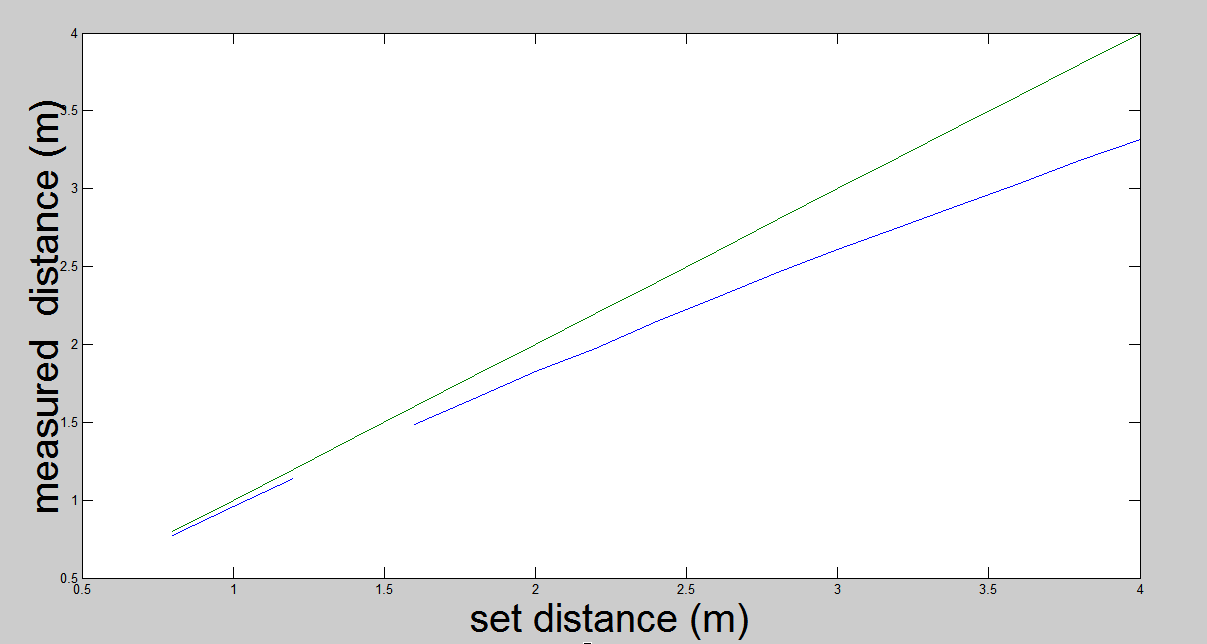
\includegraphics[width = 0.8\textwidth]{avDist}
	\end{center}
	\caption{Measured distance vs set distance. This is the average of all the pixels in the frames at a range of distances, the blue line shows the data. Green shows the target line.}
	\label{fig:avDist}
\end{figure}

Now with the clean data we know that all the data points must belong to a plane with distance to the plane being the calibration distance. For now we assume that the x and y directions are not in need of calibration, as objects in the visualisations do not too distorted in these directions. Therefore we only need to find the difference between measured data and the calibration distance. Mapping these correction vectors into a 3D space that later we can look up in to correct new data. 

In order to have the 3D correction field be continuous we must smooth and interpolate the data in all 3 dimensions. One significant issue is that all of our correction vectors fall into quite thin regions in the 3D space along the z axis, and within those areas the data is very dense in the x and y dimensions. Therefore our task is to preform smoothing in the x and y directions to remove the signal noise and to find a good interpolation scheme looking in the z direction. The interpolation should be smooth to avoid damaging the flatness of planes. 

In order to avoid large computation times on the embedded device it is important that we must invert the correction function. As it stands for each data point at the input we would have to search for the two closest calibration measurements for that pixel doing this for every pixel will be very time consuming. With an inverted correction lookup table it is possible to go directly to the correct entries in the table. Assuming we would have done the search on each pixel using binary search, this is a saving of at least 3 times for this section of the algorithm. 

\subsection{Results of calibration} % (fold)
 \label{sub:results_of_calibration}
 After performing the calculations described above we are left with 19200 look up tables (one for each pixel), each of these contain the real depth value for a given depth measurement. This correction lookup was applied to the point cloud data of uninterrupted planes. The results are very good, Figure~\ref{fig:beforeAfter} shows the point cloud data before and after correction, where both images are produced by subtracting the images average distance from all pixels and setting the dynamic range to be from -10\% of the average to +10\%. Therefore an ideal image of a plane should be a pure grey. As you can see the image before has a large area of distortion in the upper right hand corner, this is almost completely removed after correction. Table~\ref{tab:averages} shows the average distance measured over the whole plane for a range of measurements and their respective corrections, this shows that we have also corrected effectively for the absolute inaccuracy found with the Xtion sensor. 

 Figure~\ref{fig:outputTest} shows very clearly how important the calibration of the sensor was. The camera took the data points while pointing at a flat wall, a small section of orthogonal flat wall is also visible. Pre-calibration the walls are curved and the data points describing them are dispersed, this would make finding planes very difficult. After processing the image shows the walls being properly orthogonal and flat. Also the grouping of the data points to the surface is much better.


\begin{figure}[htb]
	\centering     %%% not \center
	\subfloat[Before correction]{\label{fig:preflat8}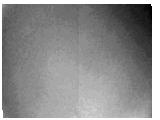
\includegraphics[width=60mm]{preflat8}} \;
	\subfloat[After correction]{\label{fig:postflat8}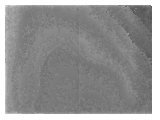
\includegraphics[width=60mm]{postflat8}}
	\caption{Example of the correction function in action. Images show divergence from the measurements average distance, white is +10\% and black is -10\% of the average respectively.}
	\label{fig:beforeAfter}
\end{figure}
\begin{figure}[htb]
	\centering     %%% not \center
	\subfloat[Before processing]{\label{fig:NewBeforeMatlab}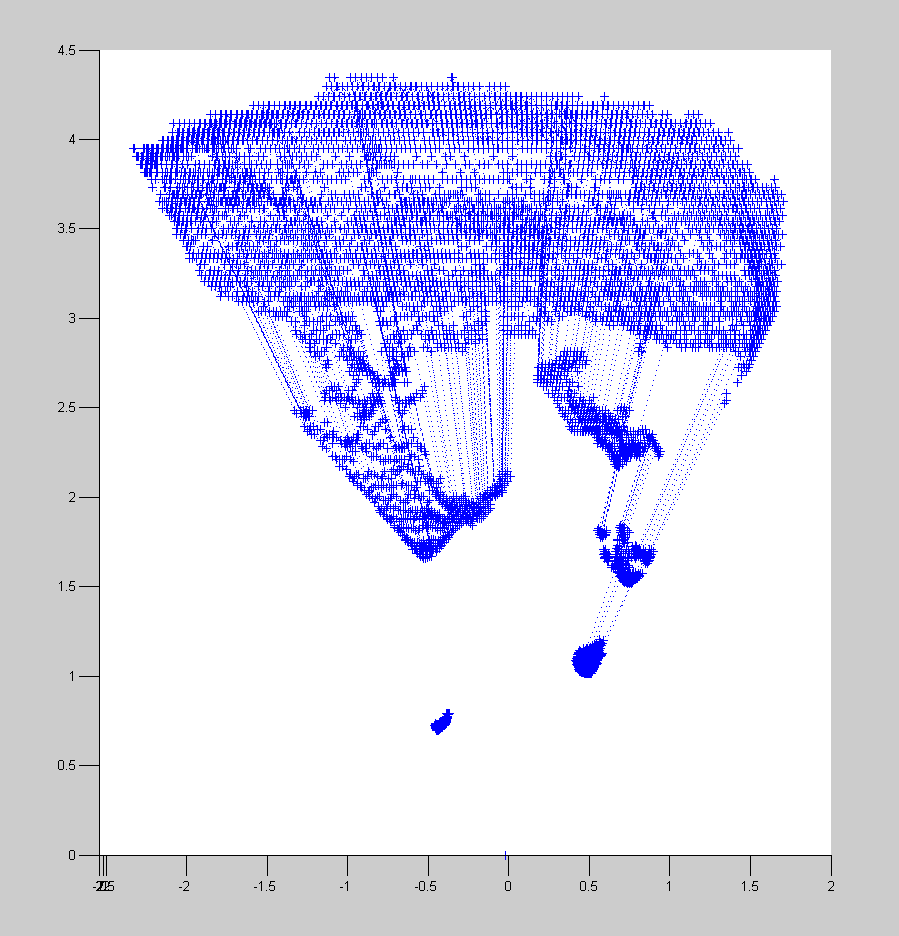
\includegraphics[width=60mm]{NewBeforeMatlab.PNG}} \;
	\subfloat[After processing]{\label{fig:NewAfterMatlab}\includegraphics[width=60mm]{NewAfterMatlab}}
	\caption{A demonstration of the correction removing curvature from the Xtion data}
	\label{fig:outputTest}
\end{figure}

\begin{figure}[htb]
	\begin{center}
	\begin{tabular}{ccc}
		\hline

		\hline
		\textbf{Set Distance}& \textbf{Measured Distance}& \textbf{Corrected Distance} \\
		\hline
		0.8		& 0.773	& 0.800\\
		1.0		& 0.960	& 1.002\\
		1.2 	& 1.138	& 1.201\\
		1.6 	& 1.483	& 1.601\\
		1.8 	& 1.655	& 1.800\\
		2.0 	& 1.826	& 2.001\\
		2.2 	& 1.976	& 2.186\\
		2.4 	& 2.146	& 2.415\\
		2.6 	& 2.299	& 2.590\\
		2.8 	& 2.465	& 2.804\\
		3.0 	& 2.614	& 2.988\\
		3.2 	& 2.751	& 3.158\\
		3.4 	& 2.895	& 3.370\\
		3.6 	& 3.045	& 3.591\\
		3.8 	& 3.198	& 3.815\\
		4.0 	& 3.341	& 3.993\\
		\hline

		\hline
	\end{tabular}
	\end{center}
	\caption{Table showing the performance of the correction function, all units in meters}
	\label{tab:averages}
\end{figure}


 % subsection results_of_calibration (end) 
\clearpage


\section{Feature Extraction} % (fold)
\label{sec:feature_extraction}

To obtain robust and consistent computer vision the open source \ac{PCL} was used as a foundation on which our vision algorithms were implemented. By levering the both well featured and documented \ac{PCL} allowed us to rapidly develop and test our algorithms in real time. 

The first feature employed from the \ac{PCL} was normal estimation. Once the Xtion passes the raw point cloud data to the \ac{PCL}, we run a kernel operator over the image which integrates over many points to obtain an estimate of the normal. By using this integral normal estimation we smooth out noisy and sporadic normal estimations which occur if normal estimates are taken for just a single point. However, by using a kernel we require an initial amount of information, and hence, for the edges of the image there are no available normal estimations as there are no neighbouring points available in each direction. Further another caveat of using this technique is the loss of high frequency normal information, such as sharp corners or edges, due to averaging (loss of high frequency information). This latter property is discovered and discussed later in the flood fill algorithm. 

A much referenced and popular algorithm for density based clustering is \ac{DBScan}, having excellent noise immunity. The basic idea is to take a point, finding all other neighbouring points within a certain neighbourhood or radius (of distance epsilon). If enough are found (decided by a threshold value $\gamma$), then we are able iteratively expand these neighbouring points, again checking if the minimum number of neighbouring points ($\gamma$) is sufficient to be considered within the same cluster. Figure~\ref{fig:dbscan} demonstrates a pass of the algorithm starting from a point within region A and clustering outward until the density of connected points becomes to small. Listing~\ref{alg:dbscan} details the full algorithm to find all densely connected regions within an image space.

\begin{figure}[bt]
	\begin{center}
		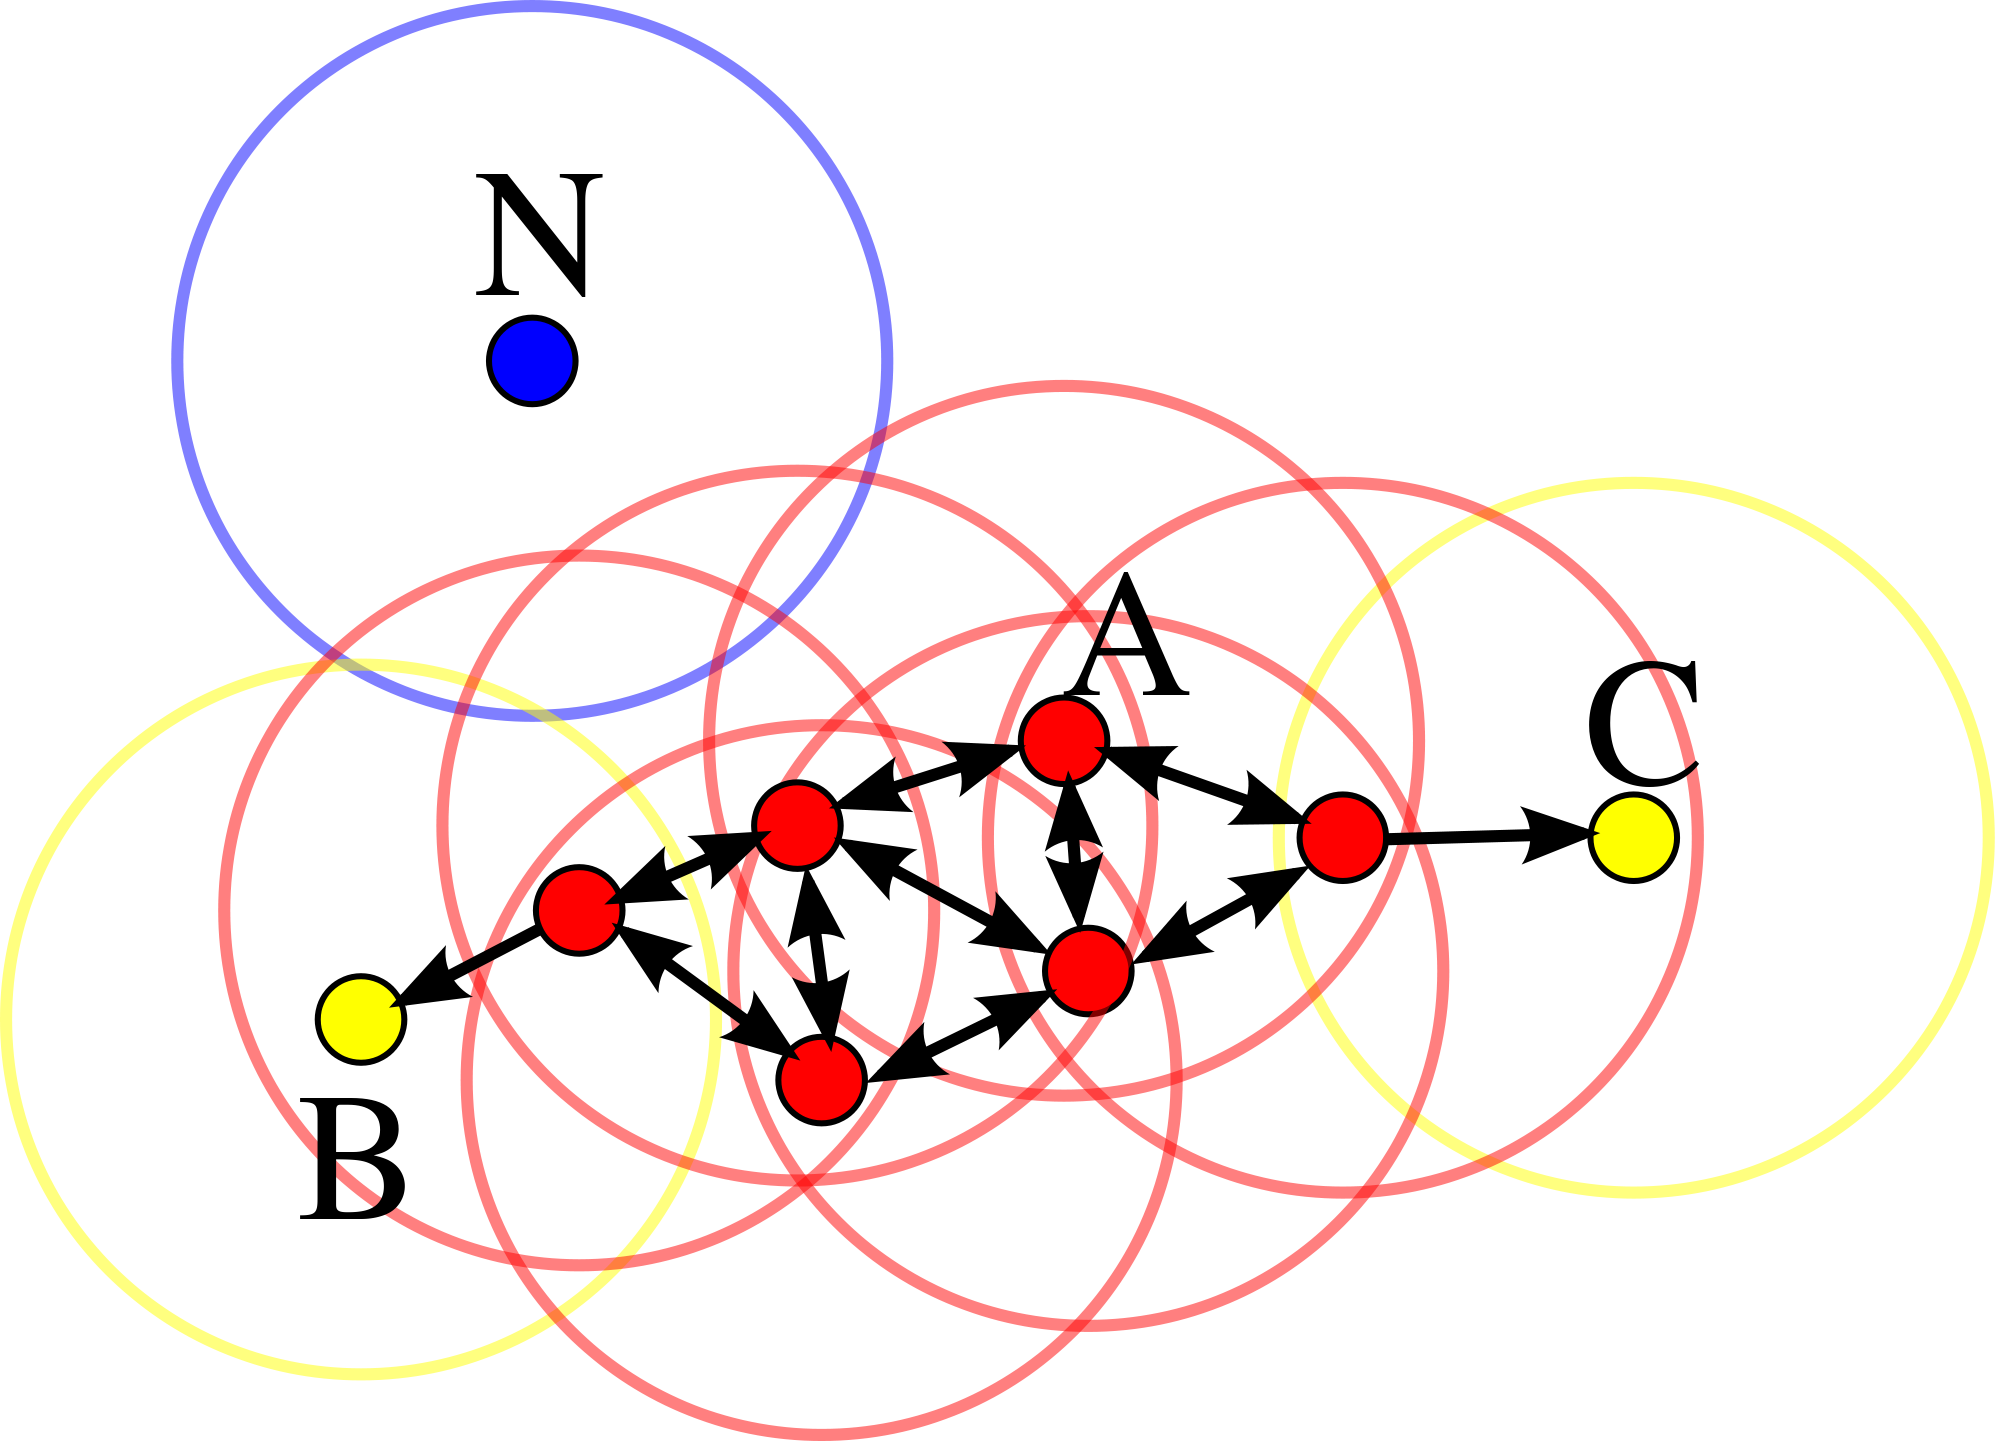
\includegraphics[width=0.6\textwidth]{2000px-DBSCAN-Illustration.png}
	\end{center}
	\caption{\ac{DBScan} clustering, starting from point within cluster A, and terminating at B and C, which do not contain enough points within their radius to be considered densely connected. N is never touched by this iteration of the algorithm as regions A, B and C are outside distance $\epsilon$.}
	\label{fig:dbscan}

\end{figure}

\begin{algorithm}[tb]
	\SetAlgoLined
	\KwData{$N \times N$ matrix: $D$}
	\KwResult{List of densely related points} 
	\bigskip
	DBScan($D$, $\epsilon$, MinPts): \\
	\ForEach {unvisited point $P$ in dataset $D$}
	{
		mark $P$ as visited; \\
		NeighbourPts $\leftarrow$ regionQuery($P$, $\epsilon$); \\
		\If{count of NeighbourPts $< \gamma$}{
			mark $P$ as noise; \\
		} 
		\Else {
			$C \leftarrow$ next cluster \\
			expandCluster($P$, NeighborPts, $C$, $\epsilon$, MinPts);
		}
	}
	\bigskip
	expandCluster($P$, NeighborPts, $C$, $\epsilon$, MinPts):  \\
	add $P$ to cluster $C$ \\
	\ForEach {point $P'$ in not visited}{
		mark $P'$ as visited; \\
		NeighbourPts' $\leftarrow$ regionQuery($P'$, $\epsilon$); \\
		\If{count of NeighbourPts' $>=$ MinPts} {
			NeighbourPts $\leftarrow$ NeighbourPts joined with NeighbourPts'; \\
		}
		\If{$P'$ is not yet a member of any cluster} {
			add $P'$ to cluster $C$'
		}
	}
	\bigskip
	regionQuery($P$, $\epsilon$):  \\
	{
 		return all points within $P'$ $\epsilon$-neighbourhood (including $P$)
	}
	\bigskip
	\caption{\ac{DBScan} pseudo code}
	\label{alg:dbscan}
\end{algorithm}

We began with a basic naïve implementation which iteratively looped through each point in the cloud, discovering all further points in x, y, z space that are within a certain distance  $(\epsilon)$. This procedure is listed as region query in algorithm~{alg:dbscan}.



We then moved onto performing the region query in normal space, meaning planes with a similar normal equation would appear in the same cluster, shown in Figure~\ref{fig:dbscan_planes}



Four parameters are required to uniquely characterize planes $(N_A, N_B, N_C, D)$ so finally we combined both the normal space with distance space (z) for the region query criteria. To make things easier, as soon as an Xtion capture becomes available, we convert the data cloud to a plane cloud (a large list containing the 4 plane parameters).

We made modifications to the DBScan algorithm to decrease the running time. By using tag fields to set whether points had already been visited or were already part of a cluster (a point can belong to one cluster only), we prevented the region query being performed superfluously. Further we built a custom conditional insertion procedure to insert into a list-like data structure without duplication, decreasing the complexity of insertion from $O(m \cdot log(n))$ (if using the \"set\" STL template class) to $O(m)$.

The DBScan algorithm completes in $O(n^2)$ if the region query completes in $O(n)$, and $O(n \cdot log(n))$ if the region query completes within $O(log(n))$. Our implementation lay somewhere between the two, having a complexity dependent on run time, where a field of view containing more planar features took longer to process. This is because captures with large or many planar features cause the region query procedure to be invoked more often, shifting the runtime complexity towards $O(n^2)$.

To combat against the possibility of slow run-time operation, we decided to use a 2 step algorithm. A simple flood fill algorithm fills the initial field of view captured from the depth camera by flooding  (clustering) connected points which have the same plane equation (remember the point cloud is now converted to a plane cloud before the flood fill step). The flood fill will generate a new set of planes, typically of a count less than 10. This will then be passed to the DBScan algorithm for the second step of the two step algorithm. The DBScan is required planes generated from flood fill may be split up my objects in the field of view. Figure X demonstrates this. Thus the second step ultilises the DBScan algorithm to merge plane regions that should be connected. 

\begin{algorithm}[tbp]
	\SetAlgoLined
	\KwData{$N \times N$ matrix: $D$}
	\KwResult{List of sets of connected points} 
	\bigskip
	FloodFill($P_{seed}$, MinPts): \\
	Push $P_{seed} \rightarrow$ Q \\
	\While {Q is not empty}
	{
	 	Pop $Q \rightarrow P$ \\
		\If{$P$ plane components within $\epsilon$ tolerence of $P_{seed}$}{
		Add $P$ to set $S$ \\

		\If{$P$ not in $Q$} {
			Push $P \rightarrow Q$ \\
			\ForEach{$H$ as direction (West, East, North, South)}{

				\If{$H$ not in $Q$}{
					Push $H \rightarrow Q$
				}

			}
		}


		}
	}
	\bigskip
	\caption{Flood fill algorithm pseudo code for a single fill area}
	\label{alg:Flood fill algorithm pseudocode for a single fill area}
\end{algorithm}

This design leads to increased throughput as the flood fill deals with the raw data from CCD space, converting 19200 points to only a few planes. The DBScan, having complexity towards a greedy $O(n^{2})$, only works on the plane set generate by the flood fill algorithm, meaning the near-quadratic complexity does not dominate run time as there are much less planes than there are points. 

The flood fill algorithm is analogous to a paint bucket function in a graphical editing package. We randomly take a seed point in pixel space (that is we randomly select a point from the depth camera output) and take the normal and distance (plane space), and then proceed to fill out from this point in all directions until the planes parameters $(N_A, N_B, N_C, D)$ differ by value epsilon from the original seed point. We continue to attempt clustering planes until either we flood a certain threshold of the image (sigma, i.e. 90\%) or have attempted to flood fill from a random seed point after a specified number of tries (gamma, i.e. 50). The flood fill algorithm works iteratively using only a simple queue structure and list keep track if points have been explored yet in the context of the current fill or already added to a previous fill (plane) respectively, resulting in a constant complexity of O(n). 

Complications arose when performing the flooding. As explained before, the projected grid from the Xtion opens in a conic fashion. This means that objects closer the Xtion will be showered in points, while those further away will contain far fewer points. This drop off happens at a quadratic rate, meaning the error in distance also occurs at a quadratic rate. To deal with this we modified the condition on the D parameter for a point to be considered within the region. As depth increases we open the parameter quadratically by projecting of the z component of the plane normal to the point z component squared. We do this for both the seed point and the point being queried. 

Therefore the conditions (which all must be satisfied) for accepting a point into the current fill region is:
\begin{align}
|P_{seed|A} - P_{A}| &< \epsilon \\
|P_{seed|B} - P_{B}| &< \epsilon\\
|P_{seed|C} - P_{C}| &< \epsilon\\
|P_{seed|D}-P_{D}| &< (|N_{seed|z} \times P^{2}_{seed|z}| + |N_{z} \times P^{2}_{z}|) \times \epsilon_{depth}
\end{align}
where as before the last equation was the same as the previous three, except changed to the D parameter.
Note that P is the point which we are testing to investigate whether it should exist in the flood region, while $P_{seed}$ is the seed point at which was first chosen to characterise the flood fill region. 

Unforeseen consequence arose from the flood fill algorithm where when the flood fill is selecting a random seed point, it can select a point near a vertex. The problem is that in order to get realistic normal components, the integral image normal estimation is an average of normals in a kernel space of 40x40 normals. This means that high frequency information is lost, as shown in Figures~\ref{fig:spurious_plane_normals} and \ref{fig:spurious_plane_normals_2}. Hence, when the flood fill algorithm is filling out, spurious long thin planes will be generated along edges, giving rise to a false positive. Initial attempts to resolve this problem by adjusting the flood fill algorithm parameters such as the minimum points to consider a plane failed.

In an effort to deal with this caveat, introducing an additional step between the Flood Fill and the DBScan which detects for false positives was undertaken. By computing the covariance matrix in XYZ space for each point in a cluster, then finding the eigenvalues of this matrix calculates the \ac{PCA} of each plane allowing us the investigate the dimensionality of each plane by checking the ratio of Eigen values generated. If there is much disparity, we can assumed that a plane has been encountered fitting to the caveat described above and hence the plane is removed from the set of planes generated by the flood fill algorithm. 

This method was never implemented as after thinking ahead towards plane association in the state update of the EKF (below), we realised that we no longer needed the DBScan algorithm or \ac{PCA}.  In fact, it was found that DBScan was no longer the algorithm suitable, but rather a similar algorithm called Iterative Nearest Neighbour (INN) should be used. This is discussed in detail in the registration section of the EKF.












\begin{figure}[tbp]
	\centering
	\subfloat[\ac{DBScan} in normal space. A total of 4 planes were found:, the floor, the white boards and two back walls] 
	{
		\label{fig:dbscan_planes}
		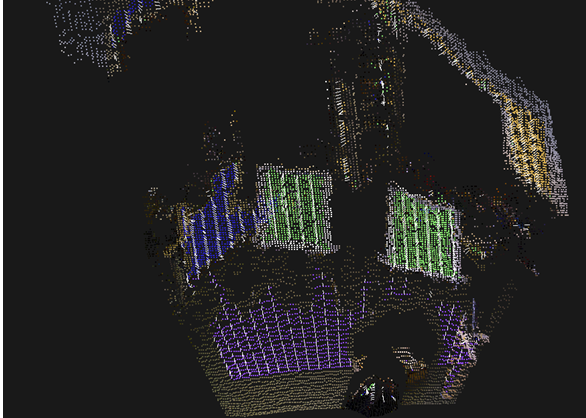
\includegraphics[width=0.8\textwidth]{6normal_boards.png}
	}

	\subfloat[\ac{DBScan} of a laboratory in xyz space. Each white board is considered a separate cluster. Distant objects coloured in blue.] {
		\label{fig:table_dbscan}
		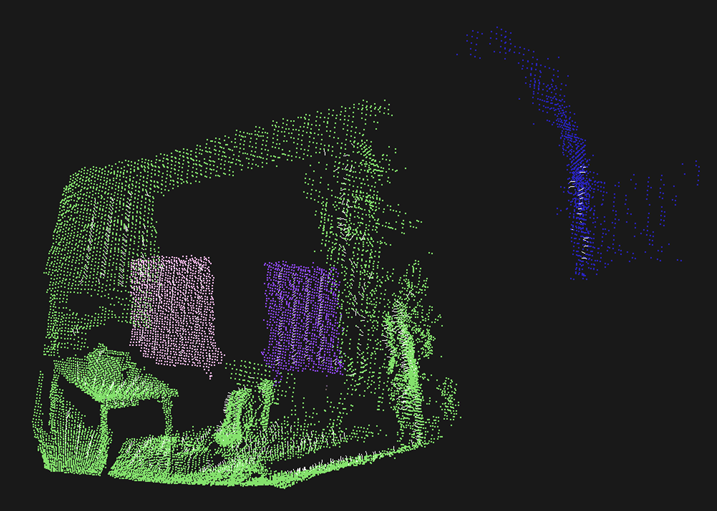
\includegraphics[width=0.8\textwidth]{6table_dbscan.png}
	}
	\caption{}
	\label{fig:DBSCAN_LAB}

\end{figure}

\begin{figure}[tbp]
	\centering     %%% not \center
	\subfloat[]{
		\label{fig:6box_before}
		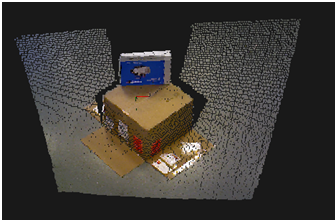
\includegraphics[width=0.45\textwidth]{6box_before.PNG}
	}
	\subfloat[]{
		\label{fig:6box_after}
		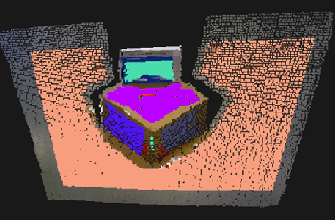
\includegraphics[width=0.45\textwidth]{6box_after.PNG}
	}

	\caption{Cluster using \ac{DBScan} in normal space}
	\label{fig:spurious_plane_normals}
\end{figure}



\begin{figure}[tbp]
	\centering     %%% not \center
	\subfloat[]{
		\label{fig:spurious_plane_normals1}
		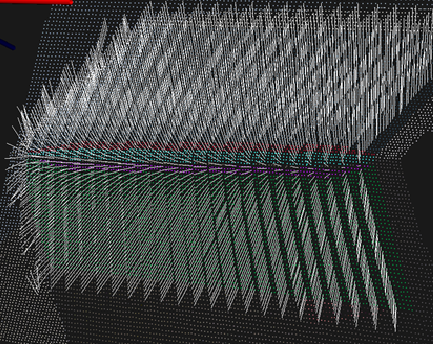
\includegraphics[width=0.45\textwidth]{6spuriousplanes_normals.PNG}
	}
	\;
	\subfloat[]{
		\label{fig:spurious_plane_normals_2}
		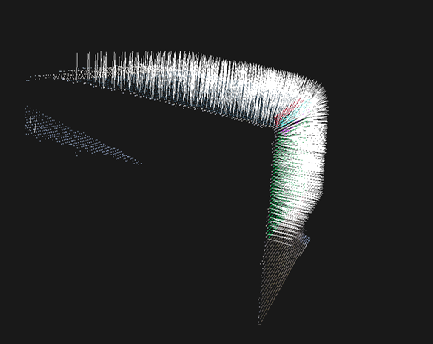
\includegraphics[width=0.45\textwidth]{6spuriousplanes_normals_2.PNG}
	}

	\caption{Normal estimation kernel causing loss of high frequency information of normals}
	\label{fig:spurious_plane_normals}
\end{figure}

% \subsection{Sensor Calibration} % (fold)
% \label{sub:sensor_calibration}

% Multidimensional least squares correction
% measure a plane at a known distance (d)
% least squares establish the observed plane that matches this distance d % 	(or just least squares the plane first??)
% the distance of each point from the plane is the true calibration vector field projected onto the normal of the observed plane (in the camera's coordinate system)
% subsection sensor_calibration (end)

% section feature_extraction (end)

\clearpage %temp!
\section{Extended Kalman Filter} % (fold)
\label{sec:ekf}

To estimate the state of the system we employ the \ac{EKF} which is the non-linear version of the regular Kalman Filter: the optimal state estimation filter \cite{todo}. When supplied with an accurate system model, and its statistical properties, the EKF provides the state estimate with the minimum mean-squared error.
The \ac{EKF} provides a near-optimal estimate of the system's state by linearising it around the current state estimate. The reason why we need the non-linear version of the filter is due to the fact that the model includes rotations, which are non-linear in nature.

% We use a kalman filter... the optimal state estimator
% non linear due to rotations -- ekf
% 	euler vs runge kutta integrator
% 		very complicated linearization equations
% 			can be overcome with unscented kalman
% 		euler is fine if sampling fast enough
% 			if deltaT is small

Our system model can be described as a six \ac{DoF} rigid body system with Newtonian mechanics. We do not model the aerodynamics of the craft and thus must rely on inertial sensors that gives information on the evolution of the system\cite{OpenPilotPaper}. The alternative would be to model the aerodynamics of the craft and the forces acting on the craft. Our approach allows us to apply our model to any system that uses the sensors because we are not concerned about the particular physiology of the agent but rather that its sensors can describe its state.
This has the advantage that modelling errors are minimised, and the time required for system identification is reduced.
Complex phenomena such as the turbulence caused by the thrust channelled around in the confined space would be close to impossible to model.

\subsection{Filter Equations} % (fold)
\label{sub:filter_equations}

The filter is based on the following discrete time update model
\begin{align}
	x_k &= f(x_{k-1}, u_{k-1}, w_{k-1}) \notag \\
	y_k &= h(x_k, v_k)
	\label{eqn:system}
\end{align}
where $x_k$ is the state vector at time $k$, $f$ is the state transition function, $u$ is the control input vector at time $k$, $w_k$ is the process noise vector at time $k$, $y_k$ is the measurement vector at time $k$, $h$ is the function that maps the state space to the observed space, and $v_k$ is the measurement noise vector.

For compartibility with the kalman filter, we assumed the noise in the system to be gaussian white noise as follows
\begin{align}
	w_k &\sim N(0,Q_k) \notag \\
	v_k &\sim N(0,R_k) \notag \\
	x_0 &\sim N(\hat{x}_0,P_0)
	\label{eqn:noisedef}
\end{align}
where $Q_k$ and $R_k$ are the process noise and measurement noise covariance matrices, at time $k$, respectively. The initial state estimate error is assumed to be drawn from a normal distribution with covariance $P_0$.

We define
\begin{align}
	\hat{x}_{k|i} 	&= \mathbb{E}[x_k|y_0 \hdots y_i] \\
	P_{k|i} 		&= \operatorname{cov}(x_k - \hat{x}_{k|i}) \notag \\
					&= \mathbb{E}[ (x_k-\hat{x}_{k|i}) (x_k-\hat{x}_{k|i})^\top | y_0 \hdots y_i]
\end{align}
where $\hat{x}_{k|i}$ is the state estimate at time $k$ given observations of the system output up to and including time $i$, and $P_{k|i}$ is the covariance matrix associated with the error of the state estimate at time $k$ given given observations of the system output up to and including time $i$.

Given the above definitions and assumptions, we can predict the evolution of the system as follows
\begin{align}
	\hat{x}_{k|k-1} &= f(\hat{x}_{k-1|k-1}, u_{k-1}, \mathbb{E}[w_{k-1}])
	\label{eqn:predictx}
\end{align}
where we assume that the noise has zero mean:
\begin{align}
	\mathbb{E}[w_{k-1}] &= 0
\end{align}

We transform the state error covariance matrix using a linear approximation to the transformation imposed by the state transition function $f$ as follows:
\begin{align}
	P_{k|k-1} &\approx F_{k-1} P_{k-1|k-1} F_{k-1}^\top + G_{k-1} Q_{k-1} G_{k-1}^\top
	\label{eqn:predictP}
\end{align}
where
\begin{align}
	F_{k-1} &= \left . \frac{\partial f}{\partial x} \right \vert _{\hat{x}_{k-1|k-1},u_{k-1}} \\
	G_{k-1} &= \left . \frac{\partial f}{\partial w} \right \vert _{\hat{x}_{k-1|k-1},u_{k-1}}
\end{align}

--------------------------------------------------------------------------------

In order to correct for errors accumulated by the state transition function we incorporate corrections based on measurements made from the output of the system. To do this, we use the \ac{EKF} update equations.
%todo: more flesh here

For each measurement, we compute the expected measurement given our current state estimate using $h$, and compute the difference $z_k$, and estimate the associated covariance matrix using a linear approximation:
\begin{align}
	z_k &= y_k - h(\hat{x}_{k|k-1}, \mathbb{E}[v_k]) \\
	S_k &= \operatorname{cov}(z_k) \notag \\
		&\approx H_k P_{k|k-1} H_k^\top + R_k
\end{align}
where $P$ and $R$ are defined in equation (\ref{eqn:noisedef}), and where we assume that the noise has zero mean:
\begin{align}
	\mathbb{E}[v_k] &= 0
\end{align}
and where
\begin{align}
	H_{k} &= \left . \frac{\partial h}{\partial x} \right \vert _{\hat{x}_{k|k-1}} \\
	V_{k} &= \left . \frac{\partial h}{\partial v} \right \vert _{\hat{x}_{k|k-1}}
\end{align}

We define the Kalman gain as follows:
\begin{align}
	K_k &= P_{k|k-1} H_k^\top S_k^{-1}
\end{align}
which is the gain that yields the \ac{MMSE} estimates when used \cite{BerkelyCourse}. Using this gain, we compute the updated state estimate as follows:
\begin{align}
	\hat{x}_{k|k} 	&= \hat{x}_{k|k-1} + K_k z_k \\
	P_{k|k} 		&\approx (I - K_k H_k) P_{k|k-1}
\end{align}

% subsubsection filter_equations (end)
\clearpage

\subsection{System Model} % (fold)
\label{sub:system_model}

\begin{figure}[tb]
	\begin{center}
		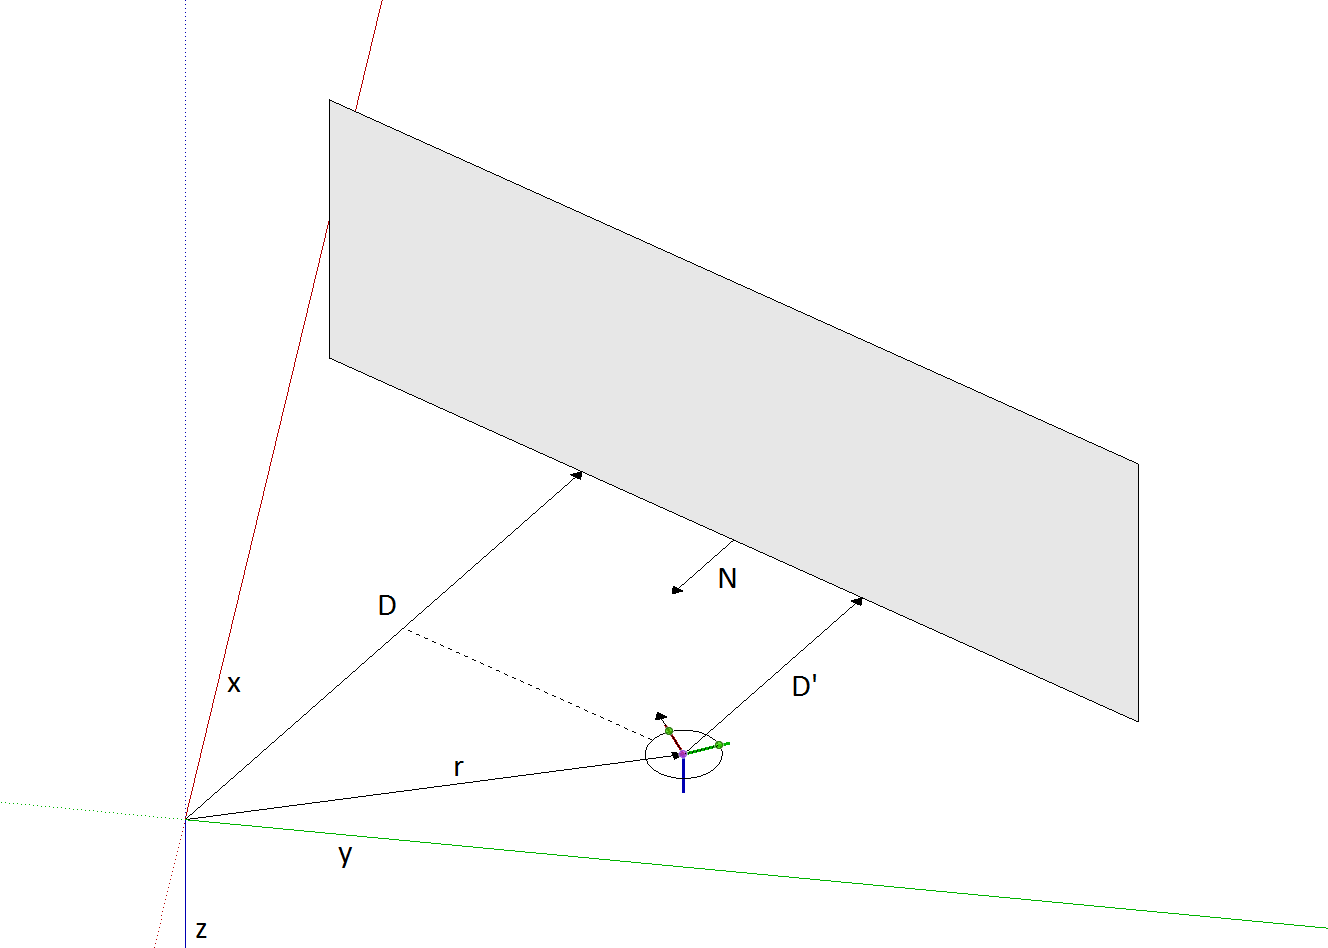
\includegraphics[width=\textwidth]{coordinatesystem.png}
	\end{center}
	\caption{The craft is located in the world coordinate system using position vector $r$, and the local coordinate axes in the body frame are depicted on the craft. A plane is represented by its normal vector, $N$ and its distance from the origin, $D$, in the world coordinate system. When observed by the craft, the plane is seen as the normal vector in the body coordinate system and the distance $D'$. It is clear from the figure that the difference between $D$ and $D'$ is the projection of $r$ along $N$.}
	\label{fig:coordinatesystem}
\end{figure}

In order to evaluate the equations from the previous section, we need to establish a model of the system. This involves establishing that 
\begin{align}
	x &=
	\left[
	\begin{matrix}
		x_r \\
		x_m
	\end{matrix}
	\right]
	=
	\left[
	\begin{matrix}
		r \\
		v \\
		q \\
		b_\omega \\
		b_a \\
		\\
		\pi_0 \\
		\vdots \\
		\pi_{n-1}
	\end{matrix}
	\right]
	&
	\dot{x} &= 
	\left[
	\begin{matrix}
		\dot{r} \\
		\dot{v} \\
		\dot{q} \\
		\dot{b}_\omega \\
		\dot{b}_a \\
		\\
		\dot{\pi}_0 \\
		\vdots \\
		\dot{\pi}_{n-1}
	\end{matrix}
	\right]
\end{align}

where $x_r$ represents the state of the craft, $x_m$ represents the state of the feature map, $r$ is the position of the craft in the inertial frame, $v$ is the velocity in the inertial frame, $q$ is the quaternion that represents the attitude of the craft: a rotation from the inertial frame to the body frame, $b_\omega$ and $b_a$ represent the gyro and accelerometer bias, respectively. $\pi_0 \hdots \pi_{n-1}$ are the equations of the planes currently stored in the map.

We also segment the $P$ matrix as suggested by \cite{Sola2013}:
\begin{align}
	P &=
	\left[
	\begin{matrix}
		P_{rr} 	& P_{rm} \\
		P_{mr} 	& P_{mm}
	\end{matrix}
	\right]
	=
	\left[
	\begin{matrix}
		P_{rr} 		& P_{r \pi_1} 		& \cdots 	& P_{r \pi_n} \\
		P_{\pi_1 r} & P_{\pi_1 \pi_1}	& \cdots 	& P_{\pi_1 \pi_n} \\
		\vdots		& \vdots 			& \ddots 	& \vdots \\
		P_{\pi_n r} & P_{\pi_n \pi_1} 	& \cdots 	& P_{\pi_n \pi_n}
	\end{matrix}
	\right]
	\label{eqn:Pparts}
\end{align}

The state vector components are each composed as follows
\begin{align}
	r &= 
	\left[
	\begin{matrix}
		x \\
		y \\
		z
	\end{matrix}
	\right]
	&
	v &=
	\left[
	\begin{matrix}
		\dot{x} \\
		\dot{y} \\
		\dot{z}
	\end{matrix}
	\right]
	&
	q &=
	\left[
	\begin{matrix}
		q_0 \\
		q_1 \\
		q_2 \\
		q_3
	\end{matrix}
	\right]
	&
	b_\omega &=
	\left[
	\begin{matrix}
		b_{\omega_x} \\
		b_{\omega_y} \\
		b_{\omega_z} 
	\end{matrix}
	\right]
	&
	b_a &=
	\left[
	\begin{matrix}
		b_{a_x} \\
		b_{a_y} \\
		b_{a_z} 
	\end{matrix}
	\right]
	&
	\pi &=
	\left[
	\begin{matrix}
		N_x \\
		N_y \\
		N_z \\
		D
	\end{matrix}
	\right]
\end{align}

The derivative of the state vector is computed in order to propagate the state over time.
\begin{align}
	\dot{r} &= v
	&
	\dot{v} &= R_{eb}(q) a
	&
	\dot{q} &= \frac{1}{2}\Xi(q) \omega
	&
	\dot{b}_\omega &= w_{b\omega}
	&
	\dot{b}_a &= w_{ba}
	&
	\dot{\pi} &= 0
\end{align}

where $a$ and $\omega$ are the true body frame accelerations and angular rates, respectively.
$R_{eb}$, the body to earth rotation matrix and $\Xi$ is the matrix that maps the body frame angular rates to the rate of change of quaternion. Both matrices are a function of the current quaternion and are defined below.

\begin{align}
	\omega &= \omega_m + w_\omega - b_\omega &
	a &= a_m + w_a - b_a + g_b
\end{align}
where $a_m$ and $\omega_m$ are the measured accelerations and angular velocities in the body frame, respectively, and $g_b$ is the acceleration due to gravity in the body frame.

The process noise is defined as defined and it represents the noise in the inertial sensors. To derive a close enough estimate of this noise, we computed the variance of a sample from the sensors at a stationary position[Insert link to code].
\begin{align}
	w &= 
	\left[
	\begin{matrix}
		w_\omega \\
		w_a \\
		w_{b\omega} \\
		w_{ba}
	\end{matrix}
	\right]
	% \omega_w0 = 
	% \begin{bmatrix}
	% 	 0.0001679  &-6.15e-05 &-0.0001051 \\
	% 	 -6.15e-05   &0.000132 & -6.54e-05\\
	% 	-0.0001051  &-6.54e-05 & 0.0002536\\
	% \end{bmatrix}
	% \right]
	% \omega_a0 = 
	% \begin{bmatrix}
	% 	 0.000667   3.77e-05  -6.48e-05 \\
	% 	 -3.77e-05  0.0008222 -0.0001422\\
	% 	--6.48e-05 -0.0001422  0.0027314\\
	% \end{bmatrix}
	% \right]
	% \omega_bw0 = 
	% \begin{bmatrix}
	% 	 0.0003552  -3.23e-05 -0.0002509 \\
	% 	 3.23e-05  0.0002822 -0.0002381\\
	% 	-0.0002509 -0.0002381  0.0005686\\
	% \end{bmatrix}
	% \right]
	% \omega_ba0 = 
	% \begin{bmatrix}
	% 	 0.003501  -0.001312   0.002149 \\
	% 	 -0.001312   0.004719  -0.002273\\
	% 	 0.002149  -0.002273    0.01367\\
	% \end{bmatrix}
	% \right]
\end{align}

$f$ in equation (\ref{eqn:system}) and (\ref{eqn:predictx}) operates in discrete time, but we have established our model in continuous time. As such, we perform a first order approximation to the continuous time system:
\begin{align}
	f &= x + \Delta T \dot{x}
	\label{eqn:descrete_f}
\end{align}

\begin{align}
	\Xi(q) &=
	\left[
	\begin{matrix}
		-q_1 	& -q_2	& -q_3 	\\
		q_0		& -q_3 	& q_2 	\\
		q_3 	& q_0 	& -q_1 	\\
		-q_2 	& q_1 	& q_0
	\end{matrix}
	\right]
\end{align}

\begin{align}
	\Omega(\omega) &=
	\left[
	\begin{matrix}
		0 			& -\omega_x 	& -\omega_y	& -\omega_z	\\
		\omega_x 	& 0 			& \omega_z 	& -\omega_y \\
		\omega_y 	& -\omega_z 	& 0 		& \omega_x 	\\
		\omega_z 	& \omega_y		& -\omega_x & 0
	\end{matrix}
	\right]
\end{align}

\begin{align}
	\dot{q} 	&= \frac{1}{2} \Omega(\omega) q \\
				&= \frac{1}{2} \Xi(q) \omega
\end{align}

The derivation of the rate of change of the quaternion with respect to angular velocity in the body frame can be found in \cite{MARSlab} (see equation 108). Note that they use the convention q = q4 + q1i + q2j + q3k, while we use the convention q0 + q1i + q2j + q3k, which is the same convention used by MATLAB's Aerospace Blockset \cite{MATLABAerospace}, and the OpenPilot implementation \cite{OpenPilotPaper}.
\begin{align}
	q &= q_0 + q_1i + q_2j + q_3k
\end{align}

Rbe (rotation of body with respect to earth)
rotmatrix here.
\begin{align}
	R_{be}(q) &=
	\left[
	\begin{matrix}
		2(q_0^2 + q_1^2) - 1 	& 2(q_1 q_2 + q_0 q_3) 	& 2(q_1 q_3 - q_0 q_2) \\
		2(q_1 q_2 - q_0 q_3) 	& 2(q_0^2 + q_2^2) - 1 	& 2(q_2 q_3 + q_0 q_1) \\
		2(q_1 q_3 + q_0 q_2)	& 2(q_2 q_3 - q_0 q_1)	& 2(q_0^2 + q_3^2) - 1
	\end{matrix}
	\right]
\end{align}

The derivation of the quaternion derived rotation matrix is also shown in \cite{MARSlab} (see equation 91)

as a rotation matrix is orthogonal, we have that
\begin{align}
	R_{eb} &= R_{be}^\top
\end{align}

Linearisation: Jacobians
Descritised system $f$ as shown in Equation~(\ref{eqn:descrete_f}).
\begin{align}
	F &= \frac{\partial f}{\partial x} \notag \\
	&=
	I + \frac{\partial \dot{x}}{\partial x} \Delta T \notag \\
	% &= 
	% I_{16+4n \times 16+4n} +
	% \left[
	% \begin{matrix}
	% 	0_{3\times3} 	& I_{3\times3} 	& 0_{3\times4} 	& 0_{3\times3} 		& 0_{3\times3} 	& 0_{3\times4n} \\
	% 	0_{3\times3}		& 0_{3\times3} 	& F_{vq}	& 0_{3\times3} 		& F_{vb_a} 	& 0_{3\times4n} \\
	% 	0_{4\times3}		& 0_{4\times3} 	& F_{qq}	& F_{qb_\omega}	& 0_{4\times3}	& 0_{4\times4n} \\
	% 	0_{3\times3}		& 0_{3\times3}	& 0_{3\times4} 	& 0_{3\times3} 		& 0_{3\times3} 	& 0_{3\times4n} \\
	% 	0_{3\times3}		& 0_{3\times3}	& 0_{3\times4} 	& 0_{3\times3}		& 0_{3\times3}	& 0_{3\times4n} \\
	% 	0_{4n\times3} 		& 0_{4n\times3} 	& 0_{4n\times4} 	& 0_{4n\times3}		& 0_{4n3\times3} 	& 0_{4n\times4n}
	% \end{matrix}
	% \right] 
	% \Delta T
	% \\
	&=
	I_{16+4n \times 16+4n} +
	%\left[
	%\begin{matrix}
	%	I_{16 \times 16} 	& 0_{16 \times 4n} \\
	%	0_{4n \times 16}	& I_{4n \times 4n}
	%\end{matrix}
	%\right]
	%+
	\left[
	\begin{matrix}
		\cdot 		& I_{3x3} 	& \cdot	 	& \cdot		 	& \cdot		& \cdot \\
		\cdot		& \cdot	 	& F_{vq}	& \cdot		 	& F_{vb_a} 	& \cdot \\
		\cdot		& \cdot	 	& F_{qq}	& F_{qb_\omega}	& \cdot		& \cdot \\
		\cdot		& \cdot		& \cdot	 	& \cdot		 	& \cdot		& \cdot \\
		\cdot		& \cdot		& \cdot	 	& \cdot			& \cdot		& \cdot \\
		\cdot		& \cdot		& \cdot	 	& \cdot			& \cdot		& \cdot
		%\dots 		& \vdots	& \vdots 	& \vdots		& \vdots	& \ddots
	\end{matrix}
	\right]
	\Delta T
	\label{eqn:F}
\end{align}
where
\begin{align}
	F_{vq} 	&= 2
	\left[
	\begin{matrix}
		F_{vq1} 	& -F_{vq0} 	& F_{vq3} 	& -F_{vq2} \\
		F_{vq2} 	& -F_{vq3} 	& -F_{vq0} 	& F_{vq1} \\
		F_{vq3} 	& F_{vq2} 	& -F_{vq1} 	& -F_{vq0}
	\end{matrix}
	\right]
\end{align}
where
\begin{align}
	F_{vq(0\cdots3)} &= \Xi(q) a
\end{align}
% that is
% \begin{align}
% 	%a &= a_m - b_a 							\notag 	\\
% 	F_{vq0} &= -q_1 a_x - q_2 a_y - q_3 a_z	\notag 	\\
% 	F_{vq1} &= q_0 a_x - q_3 a_y + q_2 a_z 	\notag	\\
% 	F_{vq2} &= q_3 a_x + q_0 a_y - q_1 a_z \notag	\\
% 	F_{vq3} &= -q_2 a_x + q_1 a_y + q_0 a_z
% \end{align}


%\begin{align}
%	&= 2
%	\left[
%	\begin{matrix}
%		q_0 a_x - q_3 a_y + q_2 a_z 	& q_1 a_x + q_2 a_y + q_3 a_z 	& -q_2 a_x + q_1 a_y + q_0 a_z 	& -q_3 a_x - q_0 a_y + q_1 a_z 	\\
%		q_3 a_x + q_0 a_y - q_1 a_z 	& q_2 a_x - q_1 a_y - q_0 a_z 	& q_1 a_x + q_2 a_y + q_3 a_z 	& q_0 a_x - q_3 a_y + q_2 a_z 	\\
%		-q_2 a_x + q_1 a_y + q_0 a_z 	& q_3 a_x + q_0 a_y - q_1 a_z 	& -q_0 a_x + q_3 a_y - q_2 a_z 	& q_1 a_x + q_2 a_y + q_3 a_z 	\\
%	\end{matrix}
%	\right]
%\end{align}

and further
\begin{align}
	F_{vb_a} &= -R_{eb}(q)
%\end{align}
&
%\begin{align}
	F_{qq}	&= \frac{1}{2} \Omega(\omega)
			 %= \frac{1}{2} \Omega(\omega_m - b_\omega)
%\end{align}
&
%\begin{align}
	F_{qb_\omega} &= -\frac{1}{2} \Xi(q)
\end{align}



We also have the Noise TODO describe (only 16x16 etc)
\begin{align}
	G &= \frac{\partial f}{\partial w} \notag \\
	&=
	\frac{\partial \dot{x}}{\partial w} \Delta T \notag \\
	&=
	\left[
	\begin{matrix}
		\cdot 			& \cdot 	& \cdot 		& \cdot \\
		\cdot 			& G_{vw_a} 	& \cdot 		& \cdot \\
		G_{qw_\omega}	& \cdot 	& \cdot 		& \cdot \\
		\cdot 			& \cdot 	& I_{3\times3}	& \cdot \\
		\cdot 			& \cdot 	& \cdot 		& I_{3\times3}
	\end{matrix}
	\right]
	\Delta T
\end{align}
where
\begin{align}
	G_{vw_a} &= R_{eb}(q)
%\end{align}
&
%\begin{align}
	G_{qw_\omega} &= \frac{1}{2} \Xi(q)
%\end{align}
%&
%\begin{align}
%	G_{b_\omega w_{b\omega}} &= I_{3x3}
%&
%	G_{b_a w_{ba}} &= I_{3x3}
\end{align}

We use a sparse matrix optimisation that is based on the fact that the plane map features do not move, as illustrated in \cite{Sola2013}.
This means that when calculating equation~(\ref{eqn:predictP}), we can use the sparsity of $F$ to simplify the calculation as follows:
\begin{align}
	F_r &= F_{(0-15,0-15)} \notag \\
	P &\leftarrow
	\left[
	\begin{matrix}
		F_r P_{rr} F_r^\top + GQG^\top 	& F_r P_{rm} \\
		P_{mr} F_r^\top 				& P_{mm}
	\end{matrix}
	\right]
\end{align}
where the parts of P are defined in equation~(\ref{eqn:Pparts}).

We also need to evaluate the error in plane observation and thus we need a function that transforms the plane in our state to the body frame. This is our inverse observation model, h.
\begin{align}
	T_h &= 
	\left[
	\begin{matrix}
		R_{be} 	& 0_{3\times1} \\
		r^\top 	& 1
	\end{matrix}
	\right]
	\\
	h &= T_h \pi
\end{align}
We also need to define H, the Jacobian of the h matrix w.r.t the state. The $H$ matrix is only a function of the robot's state and the particular plane observation in question and thus is composed of only two sections, one relating to the state, and one relating to the plane itself. As only the associated plane is relevant, only the part of the H matrix that pertains to this specific plane in the state is populated, and the other entries are set to zero.
In the implementation, we take advantage of this sparsity and compute matrix multiplication terms only related to the populated columns, as shown in \cite{Sola2013}.
\begin{align}
	\tilde{q} &= 
	\left[
	\begin{matrix}
		-q_0 \\
		q_1 \\
		q_2 \\
		q_3
	\end{matrix}
	\right]
	&
	H_{Nq(0\cdots3)} &= \Xi(\tilde{q}) N_p
\end{align}

\begin{align}
	H_{Nq} &= 2
	\left[
	\begin{matrix}
		-H_{Nq1} 	& -H_{Nq0} 	& H_{Nq3} 	& -H_{Nq2} \\
		-H_{Nq2} 	& -H_{Nq3} 	& -H_{Nq0} 	& H_{Nq1} \\
		-H_{Nq3} 	& H_{Nq2} 	& -H_{Nq1} 	& -H_{Nq0}
	\end{matrix}
	\right]
\end{align}

\begin{align}
	H &=
	\left[
	\begin{matrix}
		\begin{matrix}
			0_{3 \times 3} \\
			N_p^\top
		\end{matrix}
		& 0_{4 \times 3}
		&
		\begin{matrix}
			H_{Nq} \\
			0_{1 \times 4}
		\end{matrix}
		& 0_{4 \times 6}
		&
		%& 0
		& \cdots
		%& 0
		& T_h
		%& 0
		& \cdots
		%& 0
	\end{matrix}
	\right]
\end{align}

% subsection system_model (end)


\begin{figure}[tb]
	\begin{center}
		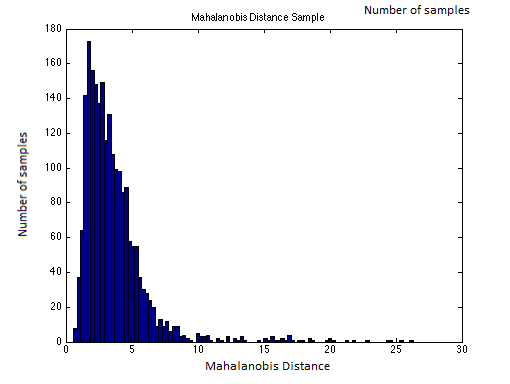
\includegraphics[width = \textwidth]{malhala_hist_100bins_10000datapoints_notmoving22}
	\end{center}
	\caption{Histogram showing the mahalanobis distance from the discovered planes to the reference planes in a stationary test with 10,000 data points.}
	\label{fig:mahaldisthist}
\end{figure}

% subsection landmark_association (end)

\subsection{Landmark Initialization} % (fold)
\label{sub:landmark_initialization}

Cool stuff from \cite{Sola2013}

\begin{align}
	y_i = 
	\left[
	\begin{matrix}
		\hat{N}_x \\
		\hat{N}_y \\
		\hat{N}_z \\
		\hat{D}
	\end{matrix}
	\right]
\end{align}

\begin{align}
	T_e &= 
	\left[
	\begin{matrix}
		R_{eb} 			& 0_{3\times1} \\
		-r^\top R_{eb}	& 1
	\end{matrix}
	\right]
\end{align}

\begin{align}
	\pi_i	&= e(y_i,x) \notag \\
			&= T_e y_i
\end{align}

\begin{align}
	x &\leftarrow
	\left[
	\begin{matrix}
		x \\
		\pi_i
	\end{matrix}
	\right]
\end{align}

\begin{align}
	E_y &= \frac{\partial e}{\partial y} \notag \\
		&= T_e \\
	E_x &= \frac{\partial e}{\partial x} \notag \\
		&=
	\left[
	\begin{matrix}
		\begin{matrix}
			0_{3 \times 3} \\
			-\hat{N}^\top R_{be}
		\end{matrix}
		&
		0_{4 \times 3}
		&
		\begin{matrix}
			E_{Nq} \\
			-r^\top E_{Nq}
		\end{matrix}
		&
		0_{4 \times 6}
	\end{matrix}
	\right]
\end{align}
where
\begin{align}
	E_{Nq} 	&= 2
	\left[
	\begin{matrix}
		E_{Nq1} 	& -E_{Nq0} 	& E_{Nq3} 	& -E_{Nq2} \\
		E_{Nq2} 	& -E_{Nq3} 	& -E_{Nq0} 	& E_{Nq1} \\
		E_{Nq3} 	& E_{Nq2} 	& -E_{Nq1} 	& -E_{Nq0}
	\end{matrix}
	\right]
\end{align}
where
\begin{align}
	E_{Nq(0\cdots3)} &= \Xi(q) \hat{N}
\end{align}

\begin{align}
	P_{\pi \pi} &= E_x P_{(0-15,0-15)} E_x^\top + E_y R E_y^\top \notag \\
	P_{x \pi} 	&= E_x P_{(0-15,all)} \notag \\
	P &\leftarrow
	\left[
	\begin{matrix}
		P 			& P_{x \pi}^\top \\
		P_{x \pi}	& P_{\pi \pi}
	\end{matrix}
	\right]
\end{align}

% subsection landmark_initialization (end)

\subsection{Landmark Association} % (fold)
\label{sub:landmark_association}
We use the statistic measurement called the mahalanobis distance to evaluate how closely a newly observed plane is related to the ones in the state map. In general the mahalanobis distance is a normalised measure that is used to identify and gauge similarity of an unknown sample to a known data set. Using this measure, we leverage the stochastic properties of our system to reduce modelling inaccuracies as opposed to using Euler distance. We use a distance threshold/ validation date such that 99\% of true measurements are accepted.. For our 4 dimensional plane measurement, this evaluates to:
$ d = chi2inv(0.99,4) = 13.2767$. In order to perform association, the procedure is we find the mahalanobis distance between our new observation and all the planes in the map, keeping the minimum. If this minimum is less than the threshold, then the data is associated, if not it is discarded as an outlier.

\subsection{Optimisation} % (fold)
\label{sub:optimisation}

SerialUpdate: \cite{OpenPilotPaper} and chapter 4.2.2 of \cite{KFBookSerialupdate}, and also mentioned in \cite{Sola2013}
The referenced papers perform an optimization which assumes an entirely uncorrelated measurement noise covariance matrix. That is the $R$ matrix is purely diagonal.
We, on the other hand, use a measurement model that includes the measurement of planes. These measurements consist of the estimated plane equation in hessian normal form. As the plane is in a three dimensional space, and thus the measurement error will have three degrees of freedom, and this form has four dimensions, the covariance matrix cannot be uncorrelated.
That is, as the hessian normal form uses a unit vector, the length of this vector is bound to unity. As such, the probability distribution of the error of the components of this normal vector cannot be spherical.
In fact, after linearisation, this distribution is projected onto a plane tangential to the actual distribution. 
%TODO: insert picture of distrubution projected onto plane

While we cannot serialise the individual components of a plane measurement, the measurement error between planes are uncorrelated, so we can still make use of the serial update strategy. As such, at each time there is a new frame that has finished feature extraction, we serially apply the measurement updates for each plane, without running the predict loop in-between.
That means the update stage will only have to invert $v$ matrices of size $4\times4$, instead of inverting a $4v \times 4v$ matrix. 
As a further optimization, we find that the equation that transforms the state covariance matrix (\ref{eqn:predictP}) forms a separable system. That is, the Jacobian matrix $F$ as defined in (\ref{eqn:F}) does not carry any information regarding the craft to the planes, and vica versa.
In fact, all terms in $F$ regarding the planes are zero, except the main diagonal, which is unity. This means that not only is it a separable system, but the plane subsystem is fully static.
Because the system is separable, and because the second half is static, we can ignore the second half of the system when computing (\ref{eqn:predictP}).
This makes an enormous difference in the scalability of the kalman filter approach. If the entire matrix-matrix multiplication is required, then the algorithm will scale like $O(n^3)$ where $n$ is the number of planes in the state vector. Now that this cubic dependence on $n$ is removed, only $O(n^2)$ terms remain, along with other terms.
%TODO: explore complexity
%TODO: incorporate reasoning from Sola2013

	We cross check our implementation against a similar open source implementation by the OpenPilot team %\cite{OpenPilotinsgps}. \cite{Holz2011}

% subsection implementation (end)

% section ekf (end)

\section{Testing and Results} % (fold)
\label{sub:testing_kalman}
In our test setup, we based our coordinate system in a vertex of the room as origin defining the x,y and z coordinates to be along the three wall edges connected to the origin vertex. Our test system consist of Thalamus chip containing the inertial sensors and Xtion Pro taped together. To ensure a functional kalman filter, full observability of system in the x,y and z axis is needed. Thus we decided to observe three orthogonal planes formed by the wall that meet at the origin. We then initialise our state in the filter to be -2,2,2 in the x,y,z space. In practice however, the initial state will be close to but not exactly the same as in the filter. It is left to the kalman filter to converge to the real state estimate.

To properly running the kalman filter, we had to tune the observation covariance parameter since the range of values obtained by using the RANSAC algorithm was too low (in the order of $10^{-7}$). A larger value would result in the kalman relying too much on the inertial sensors while a smaller one means we trust the xtion's output more [Fig:~\ref{fig:trustXtion}]. Feature extraction has considerable random noise due to the random initial point for the DBscan algorithm. Thus trusting the camera would result in high frequency noise or fluctuations in state estimate. On the other hand, position estimate from the inertial sensors behave like low pass filtered values as it is obtained by double integrating the acceleration. Thus increasing the Xtion's uncertainty results in a lower frequency in estimate which means the filter is slow to respond. We choose an appropriate value such that our filter behaves within an optimal region based on three test as discussed in \cite{KalmanTuning} . We focus our analysis on position estimate alone because since it depends on speed and attitude change, a good position estimate is sufficient to validate our algorithm implying the other estimates are correct. 

First we checked for consistency in the kalman filter by verifying that most(ideally \textgreater 95\%) of error magnitude in the observation measurements are bounded to $\pm\sqrt{2\sigma}$. [Show results].After increasing the Xtion's uncertainty by a factor of 100, the results suggest that 100 is indeed too small. A factor of 10000 gives better results.

\begin{table}[ht]
\caption{Innovation Magnitude Bound Test(\textgreater 2500 samples used)} % title of Table
\centering % used for centering table
\begin{tabular}{c c c c} % centered columns (4 columns)
\hline\hline %inserts double horizontal lines
Variable & Case\#1 (factor = 100) & Case\#2 (factor = 10000)  \\ [0.5ex] % inserts table 
%heading
\hline % inserts single horizontal line
    Nx 	& 79.98\% 	& 99.54\%\\
    Ny 	& 80.12 	& 86.74 \\
    Nz 	& 79.84 	& 77.27 \\
    d 	& 79.91 	&	92.41 \\ [1ex] % [1ex] adds vertical space
\hline %inserts single line
\end{tabular}
\label{table:firstTest} % is used to refer this table in the text
\end{table}
In the second test, we check that it is not biased by computing the normalised innovation squared
\begin{equation}
	q_{k} = z_{k}^{T} S_(k)^{-1} z_{k}
\end{equation}
for a sequence of i trials. If the filter's assumptions are met then $q_{k}$ are each $\chi^{2}$ in 4 degrees of freedom. To test for that it is not biased, we can use the mean of the sequence,
\begin{equation}
	\bar{q} = \frac{1}{N}\sum_{k=1}^N {q_k}
\end{equation}
as a test statistic such that an ideal mean lies within a confidence interval [$r_{1}, r_{2}$] defined by our hypothesis $H_0$ that $\bar{q}$ is  $\chi_{4}^{2}$ distributed with probability $1-\alpha$. First we need to find the interval such that
\begin{equation}
P(N\bar{q}\in [r_{1}, r_{2}] | H_{0}) = 1 - \alpha 
\end{equation}
We choose $\alpha$ = 0.005 (i.e. defining a two sided 95\% confidence region). We get that
[$r_{1}, r_{2}$] = [$\chi_{4}(0.025), \chi_{4}(0.975)$] = 0.4844, 11.1433. For a factor of 10000 , we obtain $\bar{q}$ = 3.6561 which is within the confidence region.
In the third test, we verify that error is white and to do this, we performed the autocorrelation of the noise using our obtained Xtion factor of 10000. Ideally for whiteness, autocorrelation peaks at a lag of 0 and is essentially zero for all others. For large enough N, we can assume that r($\tau$) is normally distributed with mean 0 and variance $\frac{1}{N}$. Practically, we can compute the $\pm$ 2$\sigma$ gate and check that aleast 95\% of values fall within this confidence region. In our test, we obtained that percentage of innovation in Nx,Ny and Nz that satisfy are the condition are 98.40$\%$, 97.81\%, 98.35\%, respectively. Error in distance however gives 93.14\%. 
\begin{figure}[H]
	\centering     %%% not \center
	\subfloat[Nx error]{
		\label{fig:errorNx}
		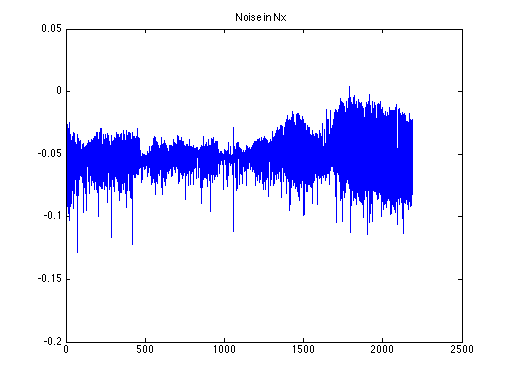
\includegraphics[width=0.45\textwidth]{noiseNx.PNG}
	}
	\;
	\subfloat[Ny error]{
		\label{fig:errorNy}
		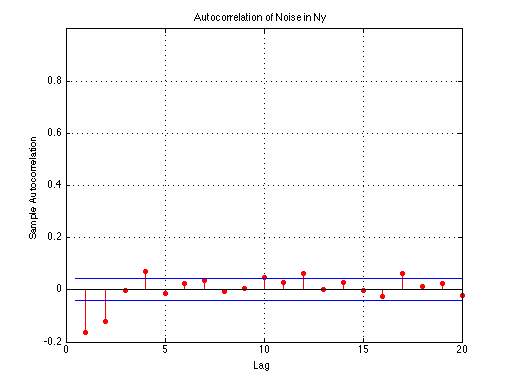
\includegraphics[width=0.45\textwidth]{noiseNy.PNG}
	}
	\;
	\subfloat[Nz error]{
		\label{fig:errorNz}
		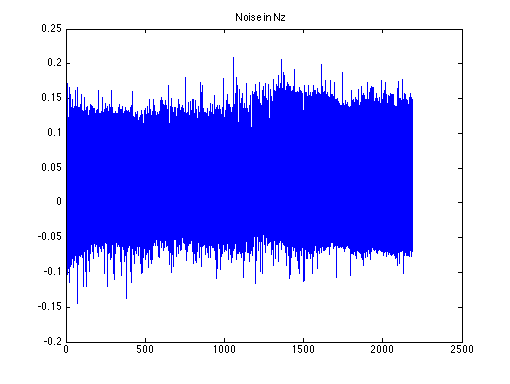
\includegraphics[width=0.45\textwidth]{noiseNz.PNG}
	}
	\;
	\subfloat[D error]{
		\label{fig:errorD}
		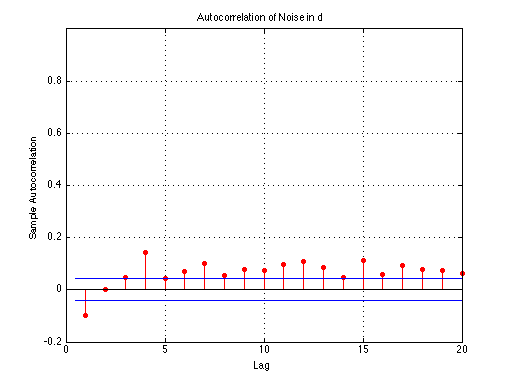
\includegraphics[width=0.45\textwidth]{noised.PNG}
	}
	\;
	\caption{Error in innovation showing whiteness expect for the distance variable}
	\label{fig:errorfigures}
\end{figure}


In order to verify that our system works with the kalman tuning, we ran it from our default initial position leaving it stationary. Below is the trajectory results. It shows a point cloud indicating that our kalman filter does indeed converge to some estimate of our real position fluctuating by only millimetres. This  somewhat accurate result is due to the full observability provided by the three orthogonal planes lying in the xy, yz, zx spaces.

\begin{figure}[H]
	\begin{center}
		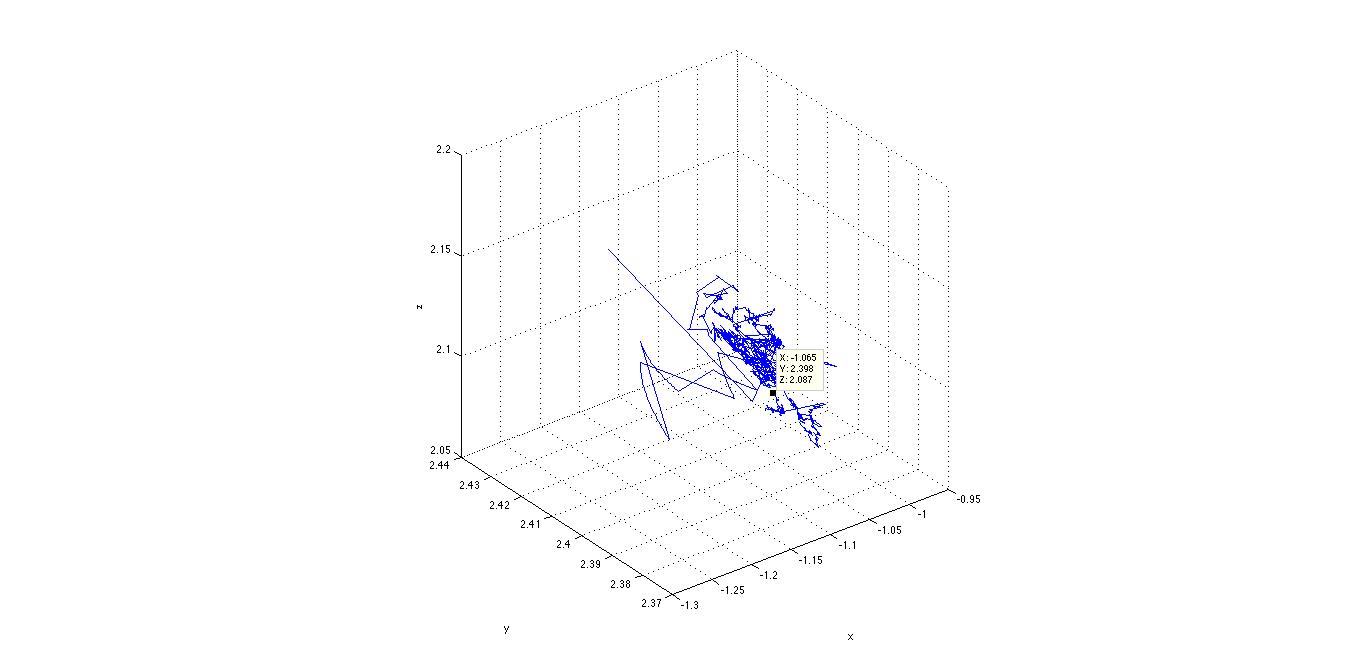
\includegraphics[width = \textwidth]{stationaryTraj.png}
	\end{center}
	\caption{Cloud point showing bounded kalman filter stationary trajectory estimation}
	\label{fig:stationary_trajectory}
\end{figure}
In the second test, we moved the setup by hand in a pseudo straight line of length 1m along across on a table in the y axis whilst ensuring that three orthogonal planes are always observed. In the figure, we see that the variation in the z axis is small as the table provided low variation in the z axis. Also, fluctuations in state estimate are in the order of millimetres.

\begin{figure}[tbh]
	\subfloat[Using an Xtion factor of 10000] {
		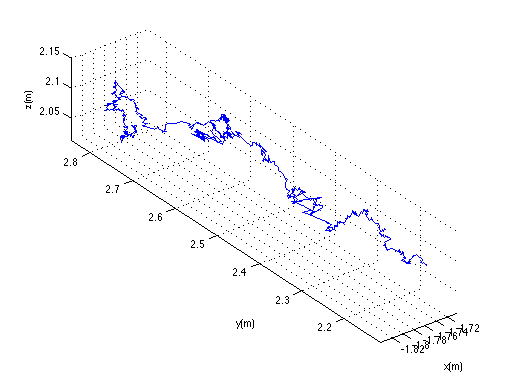
\includegraphics[width = \textwidth/2]{movingTraj.png}
	}
	\subfloat[Using an Xtion factor of 100(Higher frequency in estimation)] {
		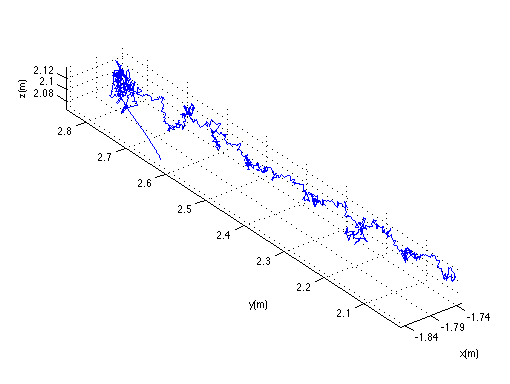
\includegraphics[width = \textwidth/2]{movingTraj100.png}
		\label{fig:trustXtion}
	}
	\caption{Cloud point showing bounded kalman filter moving trajectory estimation over a distance of 1m in the y axis}
	\label{fig:moving_trajectory}
\end{figure}

\clearpage

\section{Conclusion}


\nocite{*}

\printbibliography
% \bibliography{biblib}{}
% \bibliographystyle{plain}
% \begin{thebibliography}{99}

% \bibitem{todo}
% 	THIS REFERENCE IS MISSING!

% \bibitem{MARSlab}
% 	Nikolas Trawny and Stergios I. Roumeliotis,
% 	\emph{Indirect Kalman Filter for 3D Attitude Estimation, A Tutorial for Quaternion Algebra}. \\
% 	\url{http://www-users.cs.umn.edu/~trawny/Publications/Quaternions_3D.pdf}

% \bibitem{MATLABAerospace}
% 	MathWorks,
% 	\emph{Implement quaternion representation of six-degrees-of-freedom equations of motion with respect to body axes}. \\
% 	\url{http://www.mathworks.co.uk/help/aeroblks/6dofquaternion.html}

% \bibitem{OpenPilotPaper}
% 	Dale E. Schinstock,
% 	\emph{GPS-aided INS Solution for OpenPilot}. \\
% 	\url{http://wiki.openpilot.org/download/attachments/950387/INSGPSAlg.pdf}

% \bibitem{KFBookSerialupdate}
% 	Grewal, M.S., A.P. Andrews,
% 	\emph{Kalman Filtering, Theory and Practice Using MATLAB}. \\
% 	\url{http://www.control.aau.dk/~obin03/ESIF/Grewal,%20Andrews%20Kalman%20Filtering%20Theory%20And%20Practice%20Using%20Matlab%20(2Ed%20,%20Wiley,%202001)(410S).pdf}

% \bibitem{OpenPilotinsgps}
% 	The OpenPilot Team,
% 	\emph{Joint attitude and position estimation EKF}. \\
% 	\url{http://reviews.openpilot.org/browse/OpenPilot/flight/libraries/insgps16state.c?hb=true}

% \bibitem{ThirdYearControl}
% 	Alessandro Astolfi,
% 	\emph{Systems and Control Theory - An Introduction}. \\
% 	\url{http://www3.imperial.ac.uk/pls/portallive/docs/1/31851696.PDF}

% \bibitem{BerkelyCourse}
% 	Pieter Abbeel,
% 	\emph{Learning for robotics and control}. \\
% 	\url{http://inst.eecs.berkeley.edu/~cs294-40/fa08/#syllabus}

% \bibitem{HexCoptSelfCalb}%some interesting stuff about online sensor calibration. also quite embedded solution
% 	Stephan Weiss, Markus W. Achtelik, Margarita Chli, Roland Siegwart,
% 	\emph{Versatile Distributed Pose Estimation and Sensor
% 			Self-Calibration for an Autonomous MAV}. \\
% 	\url{http://ieeexplore.ieee.org/stamp/stamp.jsp?tp=&arnumber=6225002}

% \bibitem{KinectCopter}%very close to our solution, using kinect and atom. focus on navigation/exploration
% 	Shaojie Shen, Nathan Michael, and Vijay Kumar,
% 	\emph{Autonomous Indoor 3D Exploration with a Micro-Aerial Vehicle}. \\
% 	\url{http://ieeexplore.ieee.org/stamp/stamp.jsp?tp=&arnumber=6225146}

% \bibitem{AgresivePlane}%very close to our solution, using kinect and atom. focus on navigation/exploration
% 	Adam Bry, Abraham Bachrach, Nicholas Roy,
% 	\emph{State Estimation for Aggressive Flight in GPS-Denied Environments
% 			Using Onboard Sensing}. \\
% 	\url{http://ieeexplore.ieee.org/stamp/stamp.jsp?tp=&arnumber=6225295}

% \bibitem{CompareFilters}%Comparision between kalman and particle filter.
% Manya Afonso
% \emph{Particle Filter and Extended Kalman Filter for Nonlinear Estimation: A Comparative Study}.
%  \url{http://users.isr.ist.utl.pt/~pjcro/cadeiras/dsfps0708/SEMS/PF_EKF_TermPaper.pdf}
% \end{thebibliography}


\end{document}

